\documentclass[english]{lapesd-thesis}

% Outros \usepackage{}
\usepackage{todonotes}
\usepackage{algpseudocode}

% Níveis abaixo de \subsection não são listados no Contents
\addtocontents{toc}{\protect\setcounter{tocdepth}{2}}

%%%%%%%%%%%%%%%%%%%%%%%%%%%%%%%%%%%%%%%%%%%%%%%%%%%%%%%%%%%%%%%%%%%%
%%% Configurações da classe (dados do trabalho)                  %%%
%%%%%%%%%%%%%%%%%%%%%%%%%%%%%%%%%%%%%%%%%%%%%%%%%%%%%%%%%%%%%%%%%%%%

% Informações para capa e folha de rosto/certificacao
\titulo{Implementation of an Inter-Cluster Communication Module for Lightweight Manycore Processors in the Nanvix OS}
\autor{João Vicente Souto}
\data{1 de agosto de 2019} % ou \today
\tcc
\departamento{Departamento de Informática e Estatística}
\curso{Ciências da Computação}
\titulode{Bacharel em Ciência da Computação}
\orientador{Prof. Dr. Márcio Bastos Castro}
\afiliacaocoorientador{Universidade Federal de Santa Catarina}
\coorientador{Prof. Me. Pedro Henrique Penna}
\afiliacaocoorientador{Université de Grenoble Alpes}

% Membros da banca e coordenador
% As regras da BU agora exigem que Dr. apareça depois do nome
\membrobanca{Prof. Rômulo Silva de Oliveira, Dr.}{Universidade Federal de Santa Catarina}
\membrobanca{Prof. Odorico Machado Mendizabal, Dr.}{Universidade Federal de Santa Catarina}
% Atenção! o template da BU e o documento que apresenta as regras continua
% usando Dr antes do nome para Orientador e Coordenador!
\coordenador{Prof. Dr. Renato Cislaghi}


% Ativa indíce remissivo. Precisa estar aqui, não funciona no .cls nem no
% \BeforeBeginDocument{}
\makeindex
% Carrega definições dos acrônimos e do glossário. Isso precisa ser feito antes
% do \begin{document}

%%%%%%%%%%%%%%%%%%%%%%%%%%%%%%%%%%%%%%%%%%%%%%%%%%%%%%%%%%%%%%%%%%%%
%%% Acronyms list                                                %%%
%%%%%%%%%%%%%%%%%%%%%%%%%%%%%%%%%%%%%%%%%%%%%%%%%%%%%%%%%%%%%%%%%%%%
%%% Importante:                                      
%%% - A lista PRECISA SER MANTIDA ORDENADA
%%%%%%%%%%%%%%%%%%%%%%%%%%%%%%%%%%%%%%%%%%%%%%%%%%%%%%%%%%%%%%%%%%%%

%A
\xnewacronym[amp]{AMP}{Asymmetric Multi-Processing}
\xnewacronym[anova]{ANOVA}{Analysis of Variance}
\xnewacronym[api]{API}{Application Programming Interface}

%B

%C
\xnewacronym[cnoc]{C-NoC}{Control Network-on-Chip}
\xnewacronym[cmp]{CMP}{Chip Multiprocessor}
\xnewacronym[cow]{COW}{Copy-On-Write}
\xnewacronym[cpu]{CPU}{Central Processing Unit}

%D
\xnewacronym[dnoc]{D-NoC}{Data Network-on-Chip}
\xnewacronym[dma][longplural={Direct Memory Accesses}]{DMA}{Direct Memory Access}
\xnewacronym[dram][longplural={Dynamic Random Access Memories}]{DRAM}{Dynamic Random Access Memory}
\xnewacronym[dtlb]{DTLB}{Data Translation Lookaside Buffer}

%E

%F
\xnewacronym[flops]{FLOPS}{Floating-point Operations per Second}
\xnewacronym[fos]{FOS}{Factored Operating System}
\xnewacronym[fpga]{FPGA}{Field Programmable Gate Array}

%G
\xnewacronym[gpu]{GPU}{Graphics Processing Unit}

%H
\xnewacronym[hal]{HAL}{Hardware Abstraction Layer}
\xnewacronym[hpc]{HPC}{High-Performance Computing}

%I
\xnewacronym[iid]{i.i.d}{Independent and Identically Distributed}
\xnewacronym[ipc]{IPC}{Inter-Process Communication}
\xnewacronym[isa]{ISA}{Distributed Hash Table}
\xnewacronym[itlb]{ITLB}{Instruction Translation Lookaside Buffer}
\xnewacronym[ieee]{IEEE}{Institute of Electrical and Electronics Engineers}

%J
\xnewacronym[jtlb]{JTLB}{Join Translation Lookaside Buffer}

%K

%L
\xnewacronym[lfour]{L4}{L4 Microkernel}
\xnewacronym[ltlb]{LTLB}{Locked Translation Lookaside Buffer}

%M
\xnewacronym[mimd]{MIMD}{Multiple Instruction Multiple Data}
\xnewacronym[misd]{MISD}{Multiple Instruction Single Data}
\xnewacronym[mmio]{MMIO}{Memory-Mapped I/O}
\xnewacronym[mmu]{MMU}{Memory Management Unit}
\xnewacronym[moosca]{MOOSCA}{Manycore Operating System for Safety-Critical Application}
\xnewacronym[mos]{mOS}{multi Operating System}
\xnewacronym[mpi]{MPI}{Message Passing Interface}
\xnewacronym[mpsoc]{MPSoC}{Multiprocessor System-on-Chip}
\xnewacronym[mpu]{MPU}{Memory Protection Unit}

%N
\xnewacronym[noc]{NoC}{Network-on-Chip}
\xnewacronym[norma]{NoRMA}{No Remote Memory Access}
\xnewacronym[nos]{nOS}{Nano-Sized Operating System}
\xnewacronym[numa]{NUMA}{Non-Uniform Memory Access}

%O
\xnewacronym[os]{OS}{Operating System}

%P
\xnewacronym[pe]{PE}{Processing Element}
\xnewacronym[pgas]{PGAS}{Partitioned Global Address Space}
\xnewacronym[pmca]{PMCA}{Programmable Manycore Accelerator}
\xnewacronym[pmio]{PMIO}{Port-Mapped I/O}
\xnewacronym[posix]{POSIX}{Portable Operating System Interface}
\xnewacronym[pucminas]{PUC Minas}{Pontifical Catholic University of Minas Gerais}

%Q
\xnewacronym[qos]{QoS}{Quality of Service}

%R
\xnewacronym[rab]{RAB}{Remapping Address Block}
\xnewacronym[ram][longplural={Random Access Memories}]{RAM}{Random Access Memory}
\xnewacronym[risc]{RISC}{Reduced Instruction Set Computer}
\xnewacronym[rm]{RM}{Resource Manager}
\xnewacronym[rma][longplural={Remote Memory Accesses}]{RMA}{Remote Memory Access}
\xnewacronym[rmem][longplural={Remote Memories}]{RMem}{Remote Memory}

%S
\xnewacronym[simd]{SIMD}{Single Instruction Multiple Data}
\xnewacronym[sisd]{SISD}{Single Instruction Single Data}
\xnewacronym[shm]{SHM}{POSIX Shared Memory}
\xnewacronym[smp]{SMP}{Symmetric Multi-Processing}
\xnewacronym[soc]{SoC}{System-on-a-Chip}
\xnewacronym[spm][longplural={Software-managed Scratchpad Memories}]{SPM}{Software-managed Scratchpad Memory}
\xnewacronym[sram][longplural={Static Random Access Memories}]{SRAM}{Static Random Access Memory}
	
%T
\xnewacronym[tlb]{TLB}{Translation Lookaside Buffer}

%U
\xnewacronym[ufsc]{UFSC}{Federal University of Santa Catarina}
\xnewacronym[uga]{UGA}{University of Grenoble Alpes}
\xnewacronym[uma][longplural={Uniform Memory Accesses}]{UMA}{Uniform Memory Access}

%V
\xnewacronym[vliw]{VLIW}{Very Long Instruction Word}

%W
\xnewacronym[watts]{W}{Watts}

%%% Local Variables:
%%% mode: latex
%%% TeX-master: "main"
%%% End:

\input{init/glossary.tex}

%%%%%%%%%%%%%%%%%%%%%%%%%%%%%%%%%%%%%%%%%%%%%%%%%%%%%%%%%%%%%%%%%%%%
%%% Commands list                                                %%%
%%%%%%%%%%%%%%%%%%%%%%%%%%%%%%%%%%%%%%%%%%%%%%%%%%%%%%%%%%%%%%%%%%%%

% Writing
\newcommand{\ie}{i.e.,\xspace}
\newcommand{\eg}{e.g.,\xspace}
\newcommand{\etal}{\textit{et al.}\xspace}

% Adjetives
\newcommand{\exascale}{\textit{exascale}\xspace}

% Manycores
\newcommand{\lightweight}{\textit{lightweight}\xspace}
\newcommand{\manycore}{\textit{manycore}\xspace}
\newcommand{\manycores}{\textit{manycores}\xspace}
\newcommand{\scc}{Intel Single-Cloud Computer\xspace}
\newcommand{\xeonphi}{Intel Xeon Phi\xspace}
\newcommand{\tilegx}{Tilera TILE-Gx100\xspace}
\newcommand{\tilepro}{Tilera TILE64\xspace}
\newcommand{\mppa}{Kalray MPPA-256\xspace}
\newcommand{\taihulight}{Sunway SW26010\xspace}
\newcommand{\epiphany}{Adapteva Epiphany\xspace}
\newcommand{\optimsoc}{OpTiMSoC\xspace}
\newcommand{\hero}{HERO\xspace}
\newcommand{\arm}{ARM Cortex-A\xspace}
\newcommand{\riscv}{RISC-V\xspace}

% Architectures
\newcommand{\intel}{x86\xspace}
\newcommand{\openrisc}{OpenRISC\xspace}
\newcommand{\bostan}{Bostan\xspace}

% Operating Systems
\newcommand{\barrelfish}{Barrelfish\xspace}
\newcommand{\linux}{GNU/Linux\xspace}
\newcommand{\unix}{Unix\xspace}
\newcommand{\rtems}{RTEMS\xspace}
\newcommand{\bsd}{BSD\xspace}
\newcommand{\nodeos}{NodeOS\xspace}
\newcommand{\nanvix}{Nanvix\xspace}

% Abstractions
\newcommand{\openmp}{OpenMP}
\newcommand{\sync}{\textit{Sync}\xspace}
\newcommand{\mailbox}{\textit{Mailbox}\xspace}
\newcommand{\portal}{\textit{Portal}\xspace}

% Auxiliaries
\newcommand{\iocluster}{I/O Cluster\xspace}
\newcommand{\ioclusters}{I/O Clusters\xspace}
\newcommand{\ccluster}{Compute Cluster\xspace}
\newcommand{\cclusters}{Compute Clusters\xspace}
\newcommand{\multikernel}{\textit{Multikernel}\xspace}
\newcommand{\microkernel}{\textit{Microkernel}\xspace}

%%% Local Variables:
%%% mode: latex
%%% TeX-master: "main"
%%% End:


\begin{document}

%%%%%%%%%%%%%%%%%%%%%%%%%%%%%%%%%%%%%%%%%%%%%%%%%%%%%%%%%%%%%%%%%%%%
%%% Conteúdo                                                     %%%
%%%%%%%%%%%%%%%%%%%%%%%%%%%%%%%%%%%%%%%%%%%%%%%%%%%%%%%%%%%%%%%%%%%%

\pretextual%
% Assume-se que \pretextual já foi feito

\imprimircapa%
\imprimirfolhaderosto*
% Atenção! esse \protect é importante
\protect\incluirfichacatalografica{pre-textual/ficha.pdf}
\imprimirfolhadecertificacao

% Assume-se que \pretextual já foi feito

\begin{dedicatoria}
  Este trabalho é dedicado à wikipedia e ao stackoverflow. Essa frase está aqui apenas para testar o alinhamento e as margens
\end{dedicatoria}

%%% Local Variables:
%%% mode: latex
%%% TeX-master: "main"
%%% End:

% Assume-se que \pretextual já foi feito

\begin{agradecimentos}
  O presente trabalho foi realizado com apoio da Coordenação de Aperfeiçoamento de Pessoal de Nível Superior -- Brasil (CAPES) -- Código de Financiamento 001.
\end{agradecimentos}

%%% Local Variables:
%%% mode: latex
%%% TeX-master: "main"
%%% End:

% Assume-se que \pretextual já foi feito

\begin{epigrafe}
  If you wish to make an apple pie from scratch, \\
  you must first invent the universe. \\
  (SAGAN, C., 1980)
\end{epigrafe}

%%% Local Variables:
%%% mode: latex
%%% TeX-master: "main"
%%% End:

% Assume-se que \pretextual já foi feito

\begin{resumo}[Resumo]
	Em conjunto com a maior escalabilidade e eficiência energética, os
	\lightweight \manycores trouxeram um novo conjunto de desafios no
	desenvolvimento de software provenientes de suas particularidades
	arquiteturais. Neste contexto, sistemas operacionais tornam o
	desenvolvimento de aplicações menos onerosos, menos suscetíveis a
	erros e mais eficientes. A camada de abstração provido pelos
	sistemas operacionais suprime as características do hardware sob
	uma perspectiva simplificada e eficez. No entanto, parte dos desafios
	de desenvolvimento encontrados em \lightweight \manycores deriva
	diretamente de \textit{runtimes} e sistemas operacionais existentes,
	que não lidam completamente com a complexidade arquitetural desses
	processadores. Nós acreditamos que sistemas operacionais para a
	próxima geração de \lightweight \manycores necessitam ser repensados
	a partir de seus conceitos básicos levando em consideração as severas
	restrições arquiteturais. Em particular, as abstrações de comunicação
	desempenham um papel crucial na escalabilidade e desempenho das
	aplicações devido à natureza distribuída dos \manycores. O objetivo
	deste trabalho é propor mecanismos de comunicação entre clusters
	para o processador \manycore emergente MPPA-256. Estes mecanismos
	faz parte de uma Camada de Abstração de Hardware genérica e flexível
	para \lightweight \manycores. A Camada de Abstração de Hardware lida
	diretamente com os principais problemas encontrados no projeto de um
	sistema operacional para esses processadores. Sob estes mecanismos,
	serviços de comunicação também serão propostos para um sistema
	operacional baseado no modelo \textit{microkernel}, que busca fornecer
	um esqueleto básico para as abstrações de sistema. As contribuições
	desta dissertação estão inseridas em um contexto de pesquisa mais
	amplo, que procura investigar a criação de um sistema operacional
	distribuído baseado em uma abordagem multikernel, denominado Nanvix OS.
	O Nanvix OS se concentrará em questões de programabilidade e
	portabilidade através de um sistemas operacional compatível com o
	padrão POSIX para \lightweight \manycore. Os resultados mostraram
	a adequação dos mecanismos no comportamento esperado das abstrações
	de comunicação entre clusters.

	% Atenção! a BU exige separação através de ponto (.). Ela recomanda de 3 a 5 keywords
	\vspace{\baselineskip}
	\textbf{Palavras-chave:} HAL. Sistema Operacional Distribuído. \textit{Lightweight Manycore}. Kalray MPPA-256.
\end{resumo}

\begin{abstract}
	Jointly with further scalability and energy efficiency, \lightweight
	\manycores brought a new set of challenges in software development
	coming from their architectural particularities. In this context,
	\oss make application development less costly, less error-prone,
	and more efficient. The abstraction layer provided by \oss suppresses
	hardware characteristics from a simplified and productive perspective.
	However, part of the development challenges encountered in lightweight
	manycores stems from existing runtimes and \oss, which do not entirely
	address the complexity of these processors. We believe that \oss for the
	next generation of lightweight manycores must be redesigned from scratch
	to cope with their tight architectural constraints. In particular,
	communication abstractions play a crucial role in application scalability
	and performance due to the distributed nature of manycores. The purpose
	of this undergraduate dissertation is to propose an inter-cluster
	communication facility for the emerging manycore MPPA-256 processor.
	This facility is part of a generic and flexible \hal that deals directly
	with the key issues encountered in designing an \os for these processors.
	Above this facility, communication services will also be proposed for an
	\os based on the \textit{microkernel} model, which seeks to provide a
	basic framework for system abstractions. The contributions of this
	undergraduate dissertation are embedded in a broader research context
	that aims to investigate the creation of a distributed \os based on a
	multikernel approach, called \textit{Nanvix OS}. Nanvix OS focuses on
	programmability and portability issues for manycores through a
	POSIX-compliant \os. The results showed the adequacy of
	the mechanisms in the expected behavior of the inter-cluster
	communication abstractions.

	\vspace{\baselineskip}
	\textbf{Keywords:} HAL. Distributed Operating System. Lightweight Manycore. Kalray MPPA-256.
\end{abstract}

%%% Local Variables:
%%% mode: latex
%%% TeX-master: "main"
%%% End:


\listoffigures*  % O * evita que apareça no sumário
\listoftables*
\listoflistings*  
\listofalgorithms*

\listadesiglas*

\tableofcontents*%

%%% Local Variables:
%%% mode: latex
%%% TeX-master: "main"
%%% End:


\textual%
\glsresetall
\chapter{Introduction}
\label{ch.intro}

	% Context
	% Historical background
	% Frequency barrier
	For several years, the increase in the frequency of processors was
	employed as the main technique for achieving performance
	improvements. However, as a side effect, the temperature of
	processors started rising to high values, thus imposing a physical
	limit to the aforementioned technique. Alternatively, the constant
	improvement of semiconductor technology helped to mitigate the
	impact of this problem, allowing the industry to build more powerful
	processors with the same frequency. Therefore, knowing the
	frequency barrier and the imminent end of Moore's
	Law~\cite{moore:1965}, the academy and industry began to research
	and invest in alternatives to keep increasing the processing power
	of computer systems.

	% Improves architectural parts
	\autoref{fig:microprocessor-data} illustrates the paradigm shift
	that processors have gone through to the present day. From mid-2000,
	the frequency of processors tended to stagnate. The steady increase
	in transistors in the same chip area and the vast diversity of
	trade-offs to improve single-thread performance has softened the
	frequency impact on processors. Some significant trade-offs are
	different types of instruction sets, instruction parallelism,
	out-of-order processing techniques, branch prediction techniques,
	and various memory hierarchies. Then, in mid-2005, the performance
	of computer systems was pushed even further by increasing the number
	of processing cores in a single die. These architectures, called
	\textit{multicores}, allowed the continuous rise of the computing
	performance.

	The ever-increasing number of transistors and cores in a chip
	quickly led to the advent of \manycores. Notwithstanding, the line
	between \textit{multicores} and \manycores is very tenuous. Some
	researchers argue that the in latter architectures, losing a core it
	will not significantly impact the performance of the platform. A
	system is classified as \manycore when there is a need for
	distributed memory and on-chip networking~\cite{freitas:thesis}.

	\begin{figure}[t]
		\centering%
		\caption{Multiprocessor evolution.}%
		\label{fig:microprocessor-data}%
		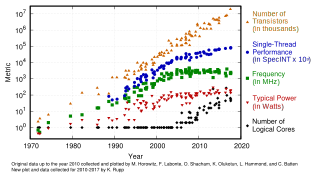
\includegraphics[width=.85\textwidth]{42-years-processor-trend.pdf}%
		\fonte{Adapted from \citeonline{url:microprocessor-trend-data}.}%
	\end{figure}

	% From multicore to manycores and Manycores characteristics
	Yet another classification for manycores is based on
	their ratio between processing speed, measured by the number of \flops, and power consumption,
	in \watts. \autoref{fig:microprocessor-data} pictures that even as the
	number of cores increasing, typical power has not grown uncontrollably.
	For instance, to achieve \exascale ($10^{18}$ \flops), the US Department
	of Defense issued a report stipulating the energy efficiency of a
	supercomputer should be around 50 GFLOPS/\watts~\cite{darpa:exascale}. 
	To cope with this energy constraint, a new class of
	parallel processors, called \lightweight \manycores, emerged to
	provide high parallelism with low power consumption.
	Lightweight manycores differ from traditional large-scale
	multicores and manycores in several points: 

	\begin{itemize}
		\item They integrate thousands of low-power cores in a single die organized in clusters;
		\item They are designed to cope with \mimd workloads;
		\item They rely on a high-bandwidth \noc for fast and reliable message-passing communication;
		\item They have constrained memory systems; and
		\item They frequently feature a heterogeneous configuration.
	\end{itemize}

	Some industry-successful examples of \lightweight \manycores are the
	\mppa~\cite{DeDinechin2013-1}; the \epiphany~\cite{olofsson2014};
	and the \taihulight~\cite{zheng2015}. Together with superior performance
	scalability and energy efficiency, lightweight manycores brought a new
	set of challenges in software development coming from their
	architectural particularities. More precisely, these 
	introduced the following difficulties:

	\begin{itemize}
		\item \textit{Hybrid programming model:} due to the parallel and
		distributed nature of the architecture, engineers are frequently
		required to adopt a message-passing programming model to deal
		with the presence of rich \nocs~\cite{kelly2013} that
		interconnects clusters and a shared-memory model inside the
		cluster;

		\item \textit{Missing hardware support for cache coherency:} to
		reduce power consumption, theses processors do not feature cache
		coherency, which in turn forces programmers to handle it
		explicitly in software level and frequently calls out for a
		redesign in their applications~\cite{francesquini2015};

		\item \textit{Constrained memory system:} the frequent presence
		of multiple physical address spaces and small local memories
		require data tiling and prefetching to be handled by the
		software~\cite{Castro2016};

		\item \textit{Heterogeneous configuration:} the different
		programmable components on \lightweight \manycores turns the
		actual deployment of applications in a complex
		task~\cite{barbalace2015}.
	\end{itemize}

	% Challenges and Problem Definition
	Part of these challenges derives from existing runtimes and \oss.
	On the one hand, runtimes do not hide the characteristics of hardware
	making software development more challenging and non-portable, \eg they
	neither allow direct access to non-local data, nor the manipulation of
	them in a transparent way. Thus, fundamental \os mechanisms, such
	as core multiplexing, core partitioning, and process and data
	migration, may not be addressed. On the other hand, the complicated
	portability and scalability of traditional \oss with a monolithic
	kernels, which were designed to homogeneous hardware, is leading to
	alternative \os designs~\cite{Baumann2009, kluge2014, nightingale2009, rhoden2011}.

	% Goals and Contributions
	We believe that \oss for the next-generation of \lightweight
	\manycores must be redesigned from scratch to cope with their tight
	architectural constraints. Based on this idea, a new fully-featured
	distributed \os based on a multikernel approach~\cite{Baumann2009}
	is under investigations~\cite{penna2017-1,penna2017-2,penna2019}.
	The \nanvix \multikernel features a generic and flexible \hal for
	\lightweight \manycores that addresses the key issues encountered in
	the development for these processors. On top of the \nanvix
	\textit{\hal}, a microkernel is being designed and implemented
	to provide the bare bones of the most important system abstractions.

\section{Goals}
\label{sec.goals}

	Based on the aforementioned motivations, the primary and specific
	goals of this work are detailed next.

\subsection{Main Goal}
\label{sec.goals.main}

	The main goal of this undergraduate dissertation is to propose an
	\textit{Inter-Cluster Communication Module} to the \nanvix
	\textit{\hal} and port it to the \mppa manycore
	processor~\cite{DeDinechin2013-1}. This module exposes the
	essential abstractions that allow overlying layers to create richer
	communication services. Using this module, we also
	propose \textit{Inter-Cluster Communication Services} to the \nanvix
	\microkernel. This work is part of the collaborative project between
	\ufsc, \pucminas, and \uga to develop an \os for \lightweight \manycore platforms.

\subsection{Specific Goals}
\label{sec.goals.specific}

	\begin{itemize}
		\item Definition and proposal of an \textit{Inter-Cluster Communication Interface} for lightweight manycores;

		\item Implementation of the proposed interface in the \nanvix \hal for the \mppa lightweight manycore processor;
        
		\item Integration of the \nanvix \hal interface with the \nanvix \microkernel;
		
		\item Performance evaluation of \nanvix \microkernel implementation using synthetic micro-benchmarks that reproduce the \textit{collective communication routines} of the \mpi programming model.
	\end{itemize}

\section{Organization Of The Work}
\label{sec.organization}
	
	The remainder of this work is organized as follows.
	\autoref{ch.fundamentation} details the background of this work.
	\autoref{ch.related-work} discusses the principal related work.
	\autoref{ch.development} presents the development of this work.
	\autoref{ch.experiments} describes the experiments accomplished and
	discusses the results. Finally, \autoref{ch.conclusions} outlines
	the main conclusions of this work.

\chapter{Theoretical Fundamentation} % Or Fundamentals?
\label{ch.fundamentation}

    In this chapter, I introduce the fundamentals concepts related to the present work.

\section{Operating Systems Concepts}
    This section may come sooner (here).

\section{Multiple Processor Systems}

    According to Tanenbaum, exists three models of modern multiple processor architectures.
    A shared-memory multiprocessor, a message-passing multicomputer, and a wide area distributed systems.
    The sections below address the two first models presenting significant hardware and software concepts for the present monograph.

    \subsection{Multiprocessors}
    Hardware overview.
    Von Neumann Model -> Main Systems Organization
    - Maybe speak UMA and NUMA.
    - Flynn's Organization.
        
    Software overview.
    - OS
    - Processor, thread (simiraly with Flynn Organization)


\subsection{Multicomputers}
    Hardware overview.
    Software overview.

    Important: Low-level Software and User-level Software primarily for communication.

\subsection{Manycores}
    Focus on manycores.

    Use the above concepts to build the narrative on manycores.

\subsubsection{MPPA-256}
    Focus on manycores.

\section{Multikernel OS Concept}
    In this section, I will write about the Multikernel OS concept using Nanvix has an example.

\section{Microkernel OS Concept}
    Focus on microkernel.

\section{Nanvix HAL}
    Focus on HAL.
\chapter{Related Work}
\label{ch.related-work}

In this chapter, we discuss related research efforts to ours.
First, we present an overview of the state-of-the-art on
\textit{\lightweight \manycore processors}. Then, due to the
lack of \oss focused on lightweight manycores, we will cover
different proposed \oss for manycores in general.

\section{Lightweight Manycore Processors}
\label{sec.works.manycores}

	Several research initiatives are focused on the design of
	\lightweight \manycores, aside from the \mppa \lightweight manycore
	processor.  For instance, \citeonline{olofsson2014} introduce
	\epiphany as a high-performance energy-efficient \manycore
	architecture suitable for real-time embedded systems.  The
	processor features multiple nodes, that communicating through three 2D mesh
	\nocs with a distributed shared-memory model without coherence
	protocol.  Each node has one \risc \cpu, multi-banked local memory,
	a \dma engine, an event monitor and a network interface.  The three
	\nocs are independent, scalable, and implement a packet-switched
	model with four duplex links at every node.

	\citeonline{Wallentowitz2013} presents the open-source \optimsoc framework
	for help and facilitate on the manycore processor design. The \optimsoc
	enables the rapid prototyping of a manycore, either via VHDL
	simulation or \fpga synthesis.
	In this architecture, several \openrisc
	core~\footnote{https://opencores.org/openrisc} are bundled into
	tiles, which in turn communicate through a \textit{packet-switched \noc}.
	The \noc support various network topologies, depending only on the tiles organization.
	Precisely, a \textit{network adapter} handles the memory transfers between
	tile and the local memory and provides a message-passing communication
	model among tiles.
	The tiles organization and the network topology allow handling
	communication by (i) message-exchange, (ii) partitioned global
	address space without cache coherence, and (iii) global memory
	with cache coherence via a write-through policy.

	Similarly, \citeonline{Kurth2017} introduces the \hero, which
	groups an \arm host processor with a fully modifiable
	\riscv \manycore implemented on an \fpga. The \pmca uses a
	multi-cluster design and relies on multi-banked memory, called \spm.
	Multi-channel \dma engines had substituted the data caches.
	Data transfer occurs between a local \spm and all remote \spms or
	with shared global memory. Communication to main memory passes
	through software-managed lightweight \rab. The \rab performs the
	translation of the virtual-to-physical address, similarly to
	traditional \mmu, allowing clusters to share virtual address pointers.

\section{Operating Systems for Manycores}
\label{sec.works.os}

	\citeonline{Baumann2009} proposed a new \os design for scalable multicore
	systems, called \multikernel.
	In their perspective, the next-generation of \oss should embrace the networked nature
	of the machines, and thus borrow design ideas from large-scale distributed
	systems.
	Assuming that cores are independent nodes of a network, they build traditional
	\os functionalities as fully-featured processes on userspace.
	These processes communicate via message-passing and do not share the internal
	structures of the \os.
	The work showed how expensive it is to maintain a state of the \os through
	shared-memory instead of exchanging messages and the subsequent increase of
	the complexity of cache-coherence protocols.
	The \multikernel implementation, named Barelfish, follows three design principles.
	First, \textit{Make all inter-core communication explicit} turns the system
	amenable to human or automated analysis because processes communicate only
	through well-defined interfaces.
	Second, \textit{Make \os structures hardware-neutral} makes the hardware-independent
	code easy to debug, optimize, and facilitates the deployment of \os for new
	processor types, avoiding rework.
	And lastly, \textit{View \os state as replicated instead of shared} improves system
	scalability.

	In \citeonline{Wisniewski2014}, the concept of scalability was pushed
	to the extreme, towards \hpc.
	The principal motivation is the creation of an \os that simultaneously supports
	programmability through support \linux \api, and provides a lightweight kernel
	to performance, scalability, and reliability.
	The \os, named \mos, provides as much of the hardware resources as
	possible to the \hpc applications and the \linux kernel component
	acts as a service that provides \linux functionalities.

	Similarly, \citeonline{kluge2014} developed the \moosca.
	With \moosca, they introduce abstractions that are easily composed, called Nodes,
	Channels, and Servers.
	Where Nodes represent execution resources, Channels represent communication
	resources, \eg \noc resources, and lastly, Servers are nodes that provide
	services to client Nodes.
	To meet safety-critical requirements, they partition \manycore and distribute
	replicas of Servers, turning the whole system more predictable.
	However, in order to deal with interferences in shared resources,
	usage policies were introduced to make possible the prediction of system behavior.

	Finally, \citeonline{nightingale2009} presents  Helios, aiming to
	simplify the task of writing, deploying, and optimizing an application across
	heterogeneous cores.
	They use the microkernel model, naming \textit{satellite kernel}, to export
	a uniform and straightforward set of \os abstractions.
	The most important design decisions were to avoid unnecessary remote communication
	by thinking about the penalty they have in \numa domains.
	Also, request the minimum of hardware primitives so that architectures with many
	constraints can be ported.
	Moreover, request the minimum hardware resources to support architectures with little
	computational power or memory constraints.

\section{Discussion}

	In \autoref{sec.works.manycores}, we discuss how \manycore architectures can be
	grouped over a common logic perspective.
	They all have one or more logical units distributed and incorporated on clusters.
	The clusters, interconnected through a network, communicate by message-exchange.
	However, due to the domain for which these processors were designed, they end up
	presenting several differences among them at the hardware level.

	Additionally, \autoref{sec.works.os} presents \oss studies that focus
	on the most efficient exploration of manycores processor characteristics.
	Many of them introduce entirely new concepts, reducing the programmability
	and portability of development environments. Some even seek to provide
	\posix interfaces by porting an adapted version of known kernels, but
	this can lead to optimization losses at near-hardware levels.
	However, the \os and communication models presented fit well with the
	distributed nature of manycores.

	In this context, \nanvix \hal deals with the lowest possible layer
	with a focus on aspects that make it challenging to work with a
	specific group of manycores, \ie \lightweight \manycores.
	The exported interfaces sought to group lightweight manycores on a common and effective view.
	Above \hal, services will be developed that seek first and foremost
	to provide greater programmability and portability through a fully-featured
	\posix-compliant \os. Besides, many of these \oss work with \numa systems,
	where a complex bus system makes communication transparent. Therefore, there
	is, in fact, no network programming. Unlike these \oss, \nanvix serves manycores
	that require explicit programming of communication through \noc. Also, features
	such as memory constraints, missing support for cache coherency, and heterogeneous
	components punctually appear in \numa architectures. The combination of these
	features makes designing an \os for \lightweight \manycores challenging.
	
\chapter{Development}
\label{ch.development}

		\todo[inline]{Need a better introducion. vvvv--- this is only copy-paste from proposal.}

	The proposal for this undergraduate dissertation is made up of two main contributions.
	The first contribution will be the port of the \textit{Inter-Cluster Communication Module},
	described in \autoref{sec.inter-cluster-communication}, for the \mppa manycore processor.
	The second contribution will be the design and implementation of communication services
	of a master-slave \os, described in \autoref{sec.communication-services}, on top of
	the inter-cluster communication module.

		\todo[inline]{Insert some paragraphs about the development, tools, etc.}

	\section{Low-Level Communication}
	\label{sec.low-level-comm}
	\todo{Or: Nanvix HAL Level}

		% O Nanvix HAL provê o módulo de comunicação inter-cluster para permitir que cluster distintos troquem informações. Esse módulo é constituido de três abstrações, nomeados Sync, mailbox e portal. Essas abstrações proveêm mecânismos mais precisos, fáceis de usar, escalonáveis e facilmente portáveis para diferentes arquiteturas~\cite{wentzlaff_fleets:_2011}. Sobre eles, é possível criar dos mais simples serviços, como sincronização e troca de dados, à serviços mais complexos como \shm, POSIX Semaphore, \rmem~\cite{penna:rmen}. O comportamento esperado pode ser simulado por ambos tipos de chamadas, sincronas ou assíncronas, dependendo apenas do suporte em hardware. Motivados a expor melhor controle sobre QoS para as camadas superiores, nós dissociamos as pequenas transferência de dados das grandes, isto é, mailbox e portal. Vale notar que seria possível utilizar uma NoC para cada abstração se o hardware suportasse. Não fizemos isso no MPPA porque a CNoC só provê a transferência de valores de 64 bits.

		% Está seção está organizada da seguinte maneira. Subseção 0 abrange pontos comuns entre todas as abstrações. Subseção 1, 2 e 3 apresentam conceitualmente cada uma das abstrações, os problemas que elas englobam, e detalhes de implementação.

		\nanvix \hal provides the inter-cluster communication module to allow separate
		clusters to exchange information.
		This module consists of three abstractions, named \sync, \mailbox, and \portal.
		These abstractions provide more precise, easy-to-use, scalable, and easily
		portable mechanisms for different architectures~\cite{wentzlaff_fleets:_2011}.
		Above them, it is possible to create from the most straightforward services, such
		as synchronization and data exchange, to more elaborate services
		like \shm, \posix Semaphore, and \rmem~\cite{penna:rmen}.
		Expected behavior can be simulated by both types of calls, synchronous or
		asynchronous, depending only on hardware support.
		Motivated to expose better \qos control to the upper layers, we decouple small data
		transfers from large ones, \ie \mailbox and \portal.
		Note that it would be possible to use an \noc for each abstraction if the hardware supported it.
		We did not do this in \mppa because \cnoc only provides the transfer of 64-bit values.
		
		This section is organized as follows.
		\autoref{sec.mppa-hardware-resources} clarifies the use of \mppa hardware resources.
		\autoref{sec.general-concepts} covers commonalities between all abstractions.
		\autoref{sec.sync-abs},
		\autoref{sec.mailbox-abs}, and
		\autoref{sec.portal-abs}
		conceptually present each of the abstractions, encompassed problems, and 
		implementation details.

		\subsection{\mppa Hardware Resources}
		\label{sec.mppa-hardware-resources}

			% A realização da comunicação de baixo-nível depende principalmente de dois recursos do MPPA, interrupções e DMA. Primeiro, o sistema de interrupções permitirá a configuração de tratadores das mensagens recebidas e enviadas através da NoC. Isto possibilitará a assíncronidade das operações, ponto vital em um sistema operacional baseado no microkernel onde o mestre não pode ficar bloqueado esperando a conclusão de uma única comunicação. Caso não fosse possível realizar pelo menos a recebimento de dados/sinais de forma assíncrona, sérios problemas de desempenho seriam introduzidos as camadas superiores. Segundo, o DMA é o mediador de todas as comunicações, síncrona ou assíncronas. Neste ponto, um hypervisor virtualiza a DMA, separando-a em duas estruturas lógicas globais, uma para a CNoC e outra para a DNoC. Cada estrutura agrupa os registradores para a configuração de envio/recebimento, e campos de bits indicando quais slots geraram uma interrupção. O hypervisor executa nos RM e controla, de forma assíncrona, as permissões de leitura/escrita dos registradores virtualizados.

			% O controle efetuado pelo hypervisor não engloba a alocação ou manipulação dos recursos. Consequentemente, nós controlamos manualmente a alocação através de campos de bits. Caso uma operação não esteja em conformidade com esse controle, é retornado um valor negativo indicando o erro, \eg alocação de um recursos que já está em uso. Assim, não inflingimos custos indesejados ao transferir a responsabilidade de tratar o erro a camada superior, \eg aguardar a liberação do recurso. A manipulação envolve procedimentos para configurar a DMA com as devidas permissões e garantir a coerência de cache das operações. Por fim, vale ressaltar que não é realizado nenhum controle de concorrência sobre as estruturas comentadas para que não seja inflingido um sobre custo sobre a abordagem do microkernel. Caso a HAL seja utilizada para desenvolver um sistema operacional monolítico, o mesmo deve se preocupar em garantir a atômicidade das operações.

			% A DMA coordena três linhas de interrupções. Duas delas são utilizados pela DNoC para notificar o recebimento de dados e o término do envio dados por uma microthread. A CNoC só utiliza uma linha para o recebimento de sinais porque o envio de um sinal, um valor de 64-bits, é realizado explicitamente pelo core. Para cada linha de interrupção existe um handler específico mas todos executam um algoritmo similar. O Algoritmo 3 exemplifica de forma simplificada o comportamento de um handler. Devido ao fato que a linha apenas notifica qual o tipo de interrupção, é responsabilidade do manipulador varrer os recursos de cada interface procurando quem acionou a interrupção. Para que não ocorresse a perda de interrupções, foi garantido que o manipulador fosse reentrante. Devido ao abordagem do microkernel, os problemas de concorrência são amenizados porque apenas o mestre trata as interrupções.

			The realization of low-level communication mainly depends on two \mppa features.
			First, the interrupt system allows the configuration of handlers for messages
			received and sent through \noc. Interrupts enable asynchronous operations,
			which is a vital point in a microkernel-based operating system where the
			master cannot be blocked waiting for a single communication to complete.
			If it were not possible to perform at least asynchronously receiving
			data/signals, upper layers would face severe performance issues. Second,
			\dma is the mediator of all communications, either synchronous or asynchronous.
			At this point, a \hypervisor virtualizes the \dma, separating it into two global
			logical structures, one for \cnoc and one for \dnoc. Each structure groups
			registers for the send/receive configuration, and bit fields indicating which
			slots generated an interrupt. The \hypervisor runs on \rms and asynchronously
			controls read/write permissions of virtualized registers.

			The control made by the \hypervisor does not include allocation or manipulation
			of resources. Consequently, we manually control allocation through bit fields.
			If an operation does not comply with this control, a negative value is returned,
			indicating the error, \eg allocation of a resource that is already in use.
			Thus, we do not inflict undesired costs by shifting responsibility for handling
			the error to the upper layer, \eg waiting for the release of a resource.
			Manipulation involves procedures for configuring the \dma with proper
			permissions and ensuring cache consistency of operations. Finally, it is
			noteworthy that there is no concurrency control over the commented
			structures so as not to inflict a cost over the microkernel approach.
			If the \nanvix \hal is used to develop a monolithic \os, it should be
			concerned with ensuring atomic operations.

			The \dma coordinates three interruption lines. Two of these are used by
			\dnoc to notify the data receipt and completion of data sending by a
			$\mu$~thread. \cnoc only uses one line for receiving signals because
			sending a signal (64-bit value) is explicitly performed by the core.
			For each interrupt line, there is a specific handler, but they all
			execute a similar algorithm. \autoref{alg.noc-handler} exemplifies
			the behavior of an \noc handler. Because the line only notifies what
			type of interrupt, it is the responsibility of the handler to search
			the resources of each interface looking for who triggered the interrupt.
			The handlers are reentrant to avoid loss of interrupts. Due to the
			microkernel approach, concurrency issues are softened because only
			the master handles interrupts.

			\begin{algorithm}[!tb]
				\caption{Simplified NoC Handler Algorithm.}%
				\label{alg.noc-handler}%
				\begin{algorithmic}[1]
					\Require $status[M_{Interfaces}][N_{Resources}]$, interrupt status of a resource.
					\Require $handlers[M_{Interfaces}][N_{Resources}]$, interrupt handler of a resource.
					\Procedure{noc\_handler}{}
					\For {$i \in [1, M_{Interfaces}]$}
						\For {$j \in [1, N_{Resources}]$}
							\If {$status[i][j] == Interrupt Triggered$}
								\State {$\Call{clean\_status}{i, j}$}
								\State {$\Call{handlers[i][j]}{i, j}$}
							\EndIf
						\EndFor
					\EndFor
					\EndProcedure
				\end{algorithmic}%
				\fonte{Developed by the Author.}%
			\end{algorithm}

			% NoC interfaces have two identifiers, one physical (physical ID) and the other logical (logical ID). The hardware uses the physical IDs in the process of data routing through \noc. Each physical ID is associated with a Logical ID to enable the identification of \noc nodes outside the \hal. Logical IDs primarily serve to disassociate the node identification from the architecture that implements the \hal. \autoref{tab.noc-node-id} shows the physical and logical identification performed for \mppa.
			% A Tabela 3 apresenta o mapeamento proposto para os clusters do MPPA. Cada linha apresenta um dos três grupos de nós NoC existentes (primeira coluna), agrupados por proximidade dos identificadores lógicos. Dentro de cada grupo temos um conjunto de identificadores físicos (segunda coluna) que são mapeados 1 para 1 para os identificadores lógicos (terceira coluna). Por exemplo, o grupo IO0 constitui 4 interfaces, onde são mapeadas da seguinte forma: $128 \to 0$, $129 \to 1$, $130 \to 2$, e $131 \to 4$. A ordem do mapeamento foi definido desta maneira para ficar mais intuitivo qual das interfaces, por consequência o cluster, é o mestre. Neste caso, o nó mestre é o identificador lógico 0, IO0. Este processo facilita na sincronização após o boot.

			\noc interfaces have two identifiers, one physical (physical ID) and the
			other logical (logical ID). The hardware uses the physical IDs in the
			process of data routing through \noc. Each physical ID is associated with
			a Logical ID to enable the identification of \noc nodes outside the \hal.
			Logical IDs primarily serve to disassociate the node identification from
			the architecture that implements the \hal. \autoref{tab.noc-node-id}
			presents the proposed mapping for \mppa clusters. Each row has one of
			three groups of existing \noc nodes (first column), grouped by type of
			the clusters. Within each group, we have a set of physical identifiers
			(second column) that are mapped 1 to 1 to logical identifiers (third column).
			For example, the \iocluster 0 constitutes 4 \noc interfaces, where they are
			mapped as follows: $128 \to 0$, $129 \to 1$, $130 \to 2$, and $131 \to 4$.
			This mapping is a more natural form to identifiers the \noc nodes through
			different architectures.

			\begin{table}[!tb]
				\centering%
				\caption{NoC Interface Identification.}%
				\label{tab.noc-node-id}%

				\begin{tabular}{l|l|l|}
					\cline{2-3}
															   & \textbf{Physical ID} & \textbf{Logical ID} \\ \hline
					\multicolumn{1}{|l|}{\textbf{\iocluster0}} & 128-131              & 0-3                 \\ \hline
					\multicolumn{1}{|l|}{\textbf{\iocluster1}} & 192-195              & 4-7                 \\ \hline
					\multicolumn{1}{|l|}{\textbf{\cclusters}}  & 0-15                 & 8-23                \\ \hline
				\end{tabular}

				\fonte{Developed by the Author.}%
			\end{table}

			% Para performar a comunicação entre dois clusters, é necessário que o emissor conheça qual o identificador do recurso que o receptor irá usar. Por exemplo, caso o receptor configurar o recebimento em um recurso da DNoC e o emissor enviar para outro, mesmo que o identificador lógico esteja correto, o receptor não será notificado do recebimento. Por esta razão, os slots de recebimento da CNoC e DNoC foram particionados por abstração. Dentro de uma partição, cada slot é mapeado estaticamente para um identificador lógico, \eg 0 à 23. Em contraste, os canais de envio não possuem essa necessidade, podendo ser alocados dinâmicamente. Entretanto, um conceito importante do Nanvix HAL é prover os recursos necessários para uma determinada operação sem realizar otimizações desnecessárias. Desta forma, os canais de envio também foram particionados por abstração de modo que sejam reservados durando toda uma operação. A tabela 3 apresenta cada abstração, identificados pelas linhas, e o particionamento dos recursos de cada NoC, identificados pelas colunas. Como a abstração sync não realiza a troca de dados arbitrários, não foram reservados recursos na DNoC. Vale notar que mesmo com a não utilização de todos os slots existentes, o aperfeiçoamento da programabilidade por não necessitar especificar os recursos de uma comunicação é um ponto forte do design das abstrações.

			The sender needs to know which logical ID the receiver will use to perform
			a communication. For instance, if the receiver sets up receiving on one
			\dnoc resource and the sender sends it to another, even if the ID is correct,
			the \dma will not notify the receiver. For this reason, the receive slots
			of the \cnoc and \dnoc have been partitioned by abstraction. Within a
			partition, each slot is statically mapped to a logical ID, \eg 0 to 23 mappings.
			In contrast, transfer channels can be dynamically allocated. However,
			an essential concept of Nanvix HAL is to provide the resources required for
			a given operation without performing additional optimizations. Thus, the
			transfer channels were also partitioned by abstraction so that they are
			reserved for an entire job. \autoref{tab.noc-resources} presents each
			abstraction, identified by the rows, and the partitioning of the resources
			of each \noc, identified by the columns. Since \sync does not exchange
			arbitrary data, no resources have been reserved in \dnoc. It is worth
			noting that even without using all existing slots, improving
			programmability by not having to specify communication features is a
			strength of abstraction design.

			% To perform the communication between two clusters, it is necessary that the
			% sender knows which resource the receiver will use.
			% For this reason, the receive slot range of \cnoc and \dnoc are partitioned
			% by abstraction, as can be seen in \autoref{tab.noc-resources}.
			% Within a partition, each slot is associated with a cluster's logical ID.
			% 	\todo{"On the another hand" does not make sense AGAIN.}
			% On the other hand, the transmitters use sending channels that need to
			% be reserved during the entire operation.
			% 	\todo{Explain the table.}
			% Thus, \autoref{tab.noc-resources} also shows the partition of the
			% sending channels for each abstraction.

			\begin{table}[!tb]
				\centering%
				\caption{Partitions of NoC resources by abstraction.}%
				\label{tab.noc-resources}%

				\begin{tabular}{l|l|l|l|l|}
					\cline{2-5}
															& \multicolumn{2}{c|}{\textbf{\cnoc}}          & \multicolumn{2}{c|}{\textbf{\dnoc}}          \\ \cline{2-5}
															& \textbf{RX Slot ID} & \textbf{TX Channel ID} & \textbf{RX Slot ID} & \textbf{TX Channel ID} \\ \hline
					\multicolumn{1}{|l|}{\textbf{\mailbox}} & 0-23                & 0                      & 0-23                & 1-3                    \\ \hline
					\multicolumn{1}{|l|}{\textbf{\portal}}  & 24-47               & 1-2                    & 24-47               & 4-7                    \\ \hline
					\multicolumn{1}{|l|}{\textbf{\sync}}    & 48-71               & 3                      & -                   & -                      \\ \hline
				\end{tabular}

				\fonte{Developed by the Author.}%
			\end{table}

			% Por fim, nós conseguimos remover quase toda dependência com a pilha de software disponibilizada pela Kalray. Porém, ao eliminar as biliotecas de comunicação, a falta de documentação da virtualização do hardware e exemplos funcionais de comunicação, surgiram limitações no envio dos dados pela DNoC. Resumidamente, não foi possível configurar corretamente as microthreads existentes na DMA para envio assíncrono, tornando-se um trabalho futuro. Entretanto, tal limitação não impactou no design das abstrações exigindo apenas que o core mestre perca um tempo enviando os dados manualmente.

			Finally, we were able to remove almost all dependency on the software
			stack provided by Kalray. However, by eliminating communication
			libraries, the lack of documentation of hardware virtualization,
			and functional examples of communication, limitations have arisen
			in the transfer of data through \dnoc. In summary, it was not possible
			to correctly configure existing $\mu$~threads in the \dma for asynchronous
			transfer, making it a future job. However, this limitation did not
			impact on the design of abstractions, requiring only that the master
			core waste time transferring data manually.

		\subsection{General Concepts of Communication Abstractions}
		\label{sec.general-concepts}

			% Tecnicamente, o Nanvix HAL não sabe que tipos de aplicações ou kernels o utilizaram. Desta forma, é preciso garantir um comportamento comum que não afete o funcionanto da camada superior. O microkernel, especificamente, restringe o core mestre a estar quase sempre disponível para atender solicitações dos escravos. Por isso, as interfaces exportam apenas chamadas assíncronas (isto é, funções async e wait). Isto força a camada superior, caso queira, criar chamadas síncronas que chamam a função wait logo após a operação assíncrona. Deste modo, no nível do microkernel, nós conseguimos garantir que o mestre configure ou execute as funções assíncronas e notifique os escravos que aguardam na função wait. No MPPA, este controle é realizado através de spinlocks atrelados a cada recurso das abstrações. Ao concluir uma operação, o mestre libera o bloqueio para o escravo continuar sua execução.

			% Contudo, a limitação da DMA descrita na Seção 0 acrescenta um agravante na operação de transferência das abstrações mailbox e portal. Nestas abstrações, existe um controle de fluxo onde o receptor deve notificar o emissor, dando-lhe permissão para transferir os dados. Este comportamento pode ocasionar o bloqueio do mestre ao esperar uma permissão. Para burlar esse problema, foi introduzido o conceito de envio preguiçoso. O algoritmo 4 ilustra o comportamento do envio preguiçoso, onde o mestre guarda os paramêtros caso não tenha permissão e vai atender outras solicitações. Ao receber a permissão do receptor, o manipulador de interrupções identifica o recurso, realiza de fato o envio dos dados e libera o escravo que solicitou o envio. Assim, nós garantimos que o mestre deixe de fazer algo útil e trave todo o sistema.

			Technically, \nanvix \hal does not know what types of applications
			or kernels have used it. Thus, we must ensure a standard behavior
			that does not affect the functionality of the upper layer. The
			microkernel specifically restricts the master core from being
			almost always available to handle slave requests. Therefore,
			interfaces export only asynchronous calls. This decision forces
			the upper layer, if desired, to create synchronous calls that
			call the wait function right after the asynchronous operation.
			Thus, at the microkernel level, we can ensure that the master
			sets or executes asynchronous functions and notifies blocked
			slaves. In \mppa, spinlocks perform synchronization between the
			master and the slaves. Upon completion of an operation, the master
			releases the lock for the slave to continue its execution.

			However, the limitation of the \dma, described in
			\autoref{sec.mppa-hardware-resources} adds an aggravation to the
			transfer operations of the mailbox and portal abstraction.
			In these abstractions, there is a flow control where the receiver
			must notify the sender, permitting him to transfer the data. This
			behavior can cause the master to lock while waiting for permission.
			The concept of lazy sending was introduced to circumvent this
			problem. \autoref{alg:lazy-transfer} illustrates the behavior of
			lazy transfer, where the master saves the parameters if not
			allowed and will handle other requests. Upon receiving permission
			from the receiver, the interrupt handler identifies the resource,
			actually sends the data and releases the slave that requested the
			send. This algorithm ensures that the master is always doing useful
			operations and never crashes the entire system.

			\begin{algorithm}[!tb]
				\caption{Simplified Lazy Transfer Algorithm.}%
				\label{alg:lazy-transfer}%
				\begin{algorithmic}[1]
				\Require $resources$, Abstraction Resource Table

				\Algphase{Configures data transfer.}

					\Procedure{async\_write}{$id, message, size$}
						\State {$resources[id].message \gets message$}
						\State {$resources[id].size \gets size$}
						\If {$resources[id].has\_permission$} 
							\State {$\Call{do\_lazy\_transfer}{id}$}
						\Else
							\State {$resources[id].is\_waiting \gets True$}
						\EndIf
					\EndProcedure%

				\Algphase{Receives permission.}

					\Procedure{abstraction\_handler}{$id$} 
						\If {$resources[id].is\_waiting$} 
							\State {$\Call{do\_lazy\_transfer}{id}$} 
						\Else
							\State {$resources[id].has\_permission \gets True$}
						\EndIf
					\EndProcedure%

				\Algphase{Transfers the data.}

					\Procedure{do\_lazy\_transfer}{$id$} 
						\State {$resources[id].is\_waiting \gets False$}
						\State {$resources[id].has\_permission \gets False$}
						\State {$\Call{transfer\_data}{resources[id].message, resources[id].size}$} 
						\State {$\Call{unlock}{resources[id].lock}$}                                \Comment{Releases slave core.}
					\EndProcedure%

				\end{algorithmic}%

				\fonte{Developed by the Author.}%
			\end{algorithm}

			% Por fim, as interfaces das abstrações seguem uma convenção para distinguir os papeis de receptor e emissor. Receptores utilizam as funções com sufíxo \texttt{create}, \texttt{unlink}, \texttt{aread} e \texttt{wait}. Emissores, por sua vez, utilizam funções com sufíxo \texttt{open}, \texttt{close}, \texttt{awrite} e \texttt{wait}. Como a função \texttt{wait} é compartilhada, a abstração deve fazer a distinção do papel pelo identificador do recurso. A diferenciação da natureza das operações ajuda tanto o usuário, sendo bastante intuitivo, como na implementação da HAL por explicitar quais recursos serão necessário.

			Finally, abstraction interfaces follow a convention to distinguish
			between receiver and sender roles. Receivers use functions with
			\texttt{create}, \texttt{unlink}, \texttt{aread}, and \texttt{wait}
			suffixes. Senders, in turn, use functions with \texttt{open},
			\texttt{close}, \texttt{awrite/signal}, and \texttt{wait} suffixes.
			Because the \texttt{wait} function is shared, the abstraction must
			distinguish the role by the resource identifier. Discriminating the
			nature of operations helps both the user, being entirely intuitive,
			and implementing HAL by explaining what features will be needed.

			% Por fim, como já comentado anteriormente, o Nanvix HAL não realiza nenhum tipo de multiplexação dos recursos físicos do hardware.
			% A quantidade de recursos de comunicação disponíveis é diretamente relativa a quantidade de recursos físico para realizar uma dada operação.
			% A tabela 4 mostra quais recursos físicos são necessário para cada abstração e a quantidade total de abstrações simultaneas que podem existir.
			% Por exemplo, a criação de um portal precisa de um slot de recebimento da DNoC e 1 canal de transmissão da CNoC.
			% As quantidades são baixas devido aos poucos canais de transmissão, porém quem deve se preocupar com a multiplexação dos recursos deve ser da camada superior.

			% \begin{table}[!tb]
			% 	\centering%
			% 	\caption{Physical requirements by abstraction.}%
			% 	\label{tab.abstractions-amount}%

			% 	\begin{tabular}{l|l|l|l|l|l|l|}
			% 		\cline{2-7}
			% 												& \multicolumn{3}{c|}{\textbf{Create}}  & \multicolumn{3}{c|}{\textbf{Open}}                              \\ \cline{2-7}
			% 												& \multicolumn{1}{|c|}{\textbf{RX}}
			% 												            & \multicolumn{1}{|c|}{\textbf{TX}}
			% 															            & \multicolumn{1}{|c|}{\textbf{Available}}
			% 																		                & \multicolumn{1}{|c|}{\textbf{RX}}
			% 																				                    & \multicolumn{1}{|c|}{\textbf{TX}}
			% 																				        			            & \multicolumn{1}{|c|}{\textbf{Available}} \\ \hline
			% 		\multicolumn{1}{|l|}{\textbf{\mailbox}} & 1 (\dnoc) & 1 (\cnoc) & 1             & 1 (\cnoc) & 1 (\dnoc) & 4                                        \\ \hline
			% 		\multicolumn{1}{|l|}{\textbf{\portal}}  & 1 (\dnoc) & 1 (\cnoc) & 2             & 1 (\cnoc) & 1 (\dnoc) & 4                                        \\ \hline
			% 		\multicolumn{1}{|l|}{\textbf{\sync}}    & 1 (\cnoc) & 0         & 24            & 0         & 1 (\cnoc) & 1                                        \\ \hline
			% 	\end{tabular}

			% 	\fonte{Developed by the Author.}%
			% \end{table}

		\subsection{Sync Abstraction}
		\label{sec.sync-abs}

			% A abstração de sincronização, chamada sync, provê o básico para a sincronização de clusters. A partir dela, é possível criar barreiras distribuidas. Seu comportamento é análogo a abstração POSIX Signals, mas as notificações não carregam informações, servem apenas para sincronização. O sync define dois modos de sincronização, ALLTOONE e ONETOALL. Nois dois modos, os clusters são separados entre um único nó mestre (ONE) e um ou mais nós escravos (ALL). A Figura 1 ilustra o modo ALLTOONE, onde o nó mestre aguarda bloqueado os N escravos realizarem a sincronização. Em contrapartida, o modo ONETOALL é utilizado quando o mestre notifica os N escravos, liberando-os do bloqueio, ilustrado pela Figura 3. Os nós emissores nunca ficam bloqueados, o trabalho deles é emitir um sinal. Os nós receptores são responsáveis por aguardar a chegada de todas as notificações.

			\textit{Synchronization Abstraction}, called \sync, provides the
			basis for cluster synchronization across distributed barriers.
			Its behavior is analogous to \posix Signals abstraction, but
			notifications do not carry information, they are only for synchronization.
			\sync defines two synchronization modes, \texttt{ALL\_TO\_ONE} and
			\texttt{ONE\_TO\_ALL}. In both modes separates the clusters between
			a single master node (\texttt{ONE}) and one or more slave nodes
			(\texttt{ALL}). \autoref{fig:sync-all-to-one} illustrates the
			\texttt{ALL\_TO\_ONE} mode, where the master node waits blocked for
			the $N$ notifications coming from the slaves. In contrast,
			\autoref{fig:sync-one-to-all} pictures the \texttt{ONE\_TO\_ALL} mode,
			where the master notifies the $N$ slaves, releasing them from the lock.
			The sender nodes are responsible for sending a signal and never will
			block. Receiver nodes are responsible for waiting for all notifications
			to arrive.

			\begin{figure}[!tb]
				\centering%
				\caption{Synchronization Abstraction Example.}%
				\label{fig:sync-concepts}%

				\subcaptionminipage[fig:sync-all-to-one]%
					{.45\linewidth}%
					{N Slaves notify the Master (\texttt{ALL\_TO\_ONE}).}%
					{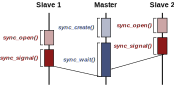
\includegraphics[width=\linewidth]{sync-all-to-one.pdf}}%
				\hspace{1cm}%
				\subcaptionminipage[fig:sync-one-to-all]%
					{.45\linewidth}%
					{The Master notifies N Slaves (\texttt{ONE\_TO\_ALL}).}%
					{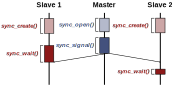
\includegraphics[width=\linewidth]{sync-one-to-all.pdf}}%

				\fonte{Developed by the Author.}%
			\end{figure}

			\subsubsection{Receiver Side Implementation}

% O que é a interface?
% Quais são os parâmetros para realizar uma operação?
				% O Codigo 4 apresenta a interface Sync para nós receptores proposta para o Nanvix HAL. Os parâmetros necessário para a abertura de um ponto de sincronização é uma lista de IDs lógicos, o tamanho da lista e o tipo de sincronização. A lista deve ser sempre inicializada com o ID do nó mestre, independentemente do modo. Os identificadores restantes, contando que não tenham repetição, podem estar em qualquer ordem. O tipos de sincronização são os modos descritos anteriormente definidos através de constantes. As demais funções utilizam o identificador da abstração retornado pela função de criação. Caso algum parâmetro esteja em desacordo ou inválido, um valor negativo é retornado indicando o erro, \eg, \texttt{nodes == NULL}.

				\autoref{code:hal-sync-receiver} introduces the Sync Interface for
				Receiver Nodes proposed for the \nanvix \hal. The parameters required
				for creating a sync point are a list of logical IDs, list size,
				and mode of synchronization. The list must always be initialized
				with the master node ID, regardless of mode. The remaining identifiers,
				provided they have no repetition, can be in any order. The other
				functions use the abstraction identifier returned by the create
				function. If any parameters are in disagreement or invalid, a
				negative value is returned indicating the error, \eg nodes pointer
				equal to \texttt{NULL}.

\begin{listing}[!tb]
\caption{Nanvix HAL: Sync Interface for Receiver Node.}
\label{code:hal-sync-receiver}
\begin{minted}{c}
/**
 * @brief Allocates and configures the receiving side of
 * the synchronization point.
 */
int sync_create(const int *nodes, int nnodes, int mode);

/* @brief Releases and cleans receiver slot. */
int sync_unlink(int syncid);

/* @brief Waits a signal. */
int sync_wait(int syncid);
\end{minted}
\fonte{Developed by the Author.}
\end{listing}

% Quais recursos são necessário para cada tipo de operação, envio e recebimento?
				% O recebimento das notificações requer a reserva 1 slot rx da CNoC relativo ao identificador do mestre. Deste modo, eliminamos o conflito no uso de diferentes slots por diferentes configurações de sincronização. Em contrapartida, um nó não poderá ser o mestre em duas operações simultâneas. O total de abstrações que podem ser criadas desta maneira é igual a quantidade de nós existentes (24 no MPPA). Nos cluster I/O, este total é multiplicado pelo número de interface NoC disponíveis, ou seja, 24 por DMA. A configuração do slot é realizado através de uma máscara de 64-bits. Está mascará é construida com os IDs lógicos dos emissores de modo que os bits relativos a suas posições sejam iguais a 0. Ao receber um sinal, a DMA realiza um OR com o valor anterior. Quando todos os bits se tornarem 1's, a DMA zera todos os bits do registrador e emite uma interrupção.

% Como as operações funcionam?
				% Um vetor de estruturas internas realiza o controle das operações. Cada posição do vetor é reservado a um slot físico e guarda flags de controle, a mascará e um spinlock. Ao realizar a abertura, espera ou unlink de um sync, a HAL verifica discrepâncias nos IDs, nas flags de controle ou nos parâmetros. Por fim, o spinlock é utilizado para sincronização da operação com os núcleos escravos. Em um sistema microkernel, o core mestre configura o sync e o escravo aguarda ser liberado no spinlock. O tratador de interrupções do Sync identifica a estrutura e libera o bloqueio. A falta de coerência de cache não afeta os spinlock porque são utilizadas instruções que garantem a atomicidade que implementam o lock.

				Receipt of notifications requires booking one \cnoc receiving slot
				related to the Master ID. This relation eliminates the conflict of
				using a same slot across different synchronization settings.
				Consequently, a node cannot be the master in two simultaneous operations.
				Thus, the total of \sync created simultaneously is equal to the number
				of existing nodes, \ie 24 in \mppa. In \ioclusters, this total is
				multiplied by the number of available NoC interfaces, \ie 24 per \dma.
				A 64-bit mask, created from sender node IDs, configures the receiving
				slot. Bits positioned on nodes IDs are 0. When receiving a signal,
				\dma performs an \textit{OR-bitwise} with the previous value. When
				all bits become 1's, \dma clears the register and triggers an interrupt.

				A vector of internal structures controls the operations. Each structure
				is reserved for a physical slot and holds control flags, the initial mask,
				and a spinlock. \hal checks for discrepancies in IDs, control flags, or
				parameters when creating, waiting, or unlinking a \sync. Finally,
				the spinlock is used to synchronize the operation with slave cores.
				On a microkernel-based system, the master core configures \sync, and
				the slave waits for the spinlock release. The interrupt handler of the
				\sync identifies the structure and releases the lock. The lack of cache
				coherence does not affect spinlocks because instructions that guarantee
				the atomicity are used to implement the lock.

% Como foi resolvido o problema de multiplos nós nos IOs? PRECISA FALAR? DARIA PRA ARRUMAR ISSO NO CÓDIGO FORÇANDO QUE O ID[1] FOSSE O ID LOCAL (CASO NAO FOR O MESTRE).
				% A lista de nós foi projetada para utilizar os IDs das interfaces NoCs ao invés dos IDs dos Cluster para não desperdiçar as DMAs extras existentes nos Cluster I/O.

			\subsubsection{Sender Side Implementation}

% O que é a interface?
% Quais são os parâmetros para realizar uma operação?
				% A interface do nó emissor, apresentada pelo Código 3, utiliza os mesmo parâmetros para abertura de um sync. Ao utilizar os mesmo valores na criação e abertura, a aplicação cliente pode definir o papel do cluster simplemente definindo qual função deve ser chamada. Entretanto, tanto na criação quanto na abertura, o ID lógico local deve estar Range correto do lista. Por exemplo, um sync é aberto com o ID local como mestre mas o tipo de sincronização é definido como ALL\_TO\_ONE. Isto retornará um erro e o sync não será aberto porque o mestre deveria ser o receptor das notificações e não o emissor. O restante da implementação segue o que já foi explicado na seção anterior.

				The Sync Interface for Sender Nodes, presented by
				\autoref{code:hal-sync-sender}, uses the same create parameters for
				opening a \sync point. The standardization of parameters simplifies
				the role of a cluster in a synchronization. However, at both creation
				and opening, the local ID must be included in the list. For instance,
				a \sync opened with the local ID as master, but the mode defines
				\texttt{ALL\_TO\_ONE} behavior. This discrepancy will return an error
				because the master should be the notification receiver and not the
				sender. The rest of the implementation follows what was already
				explained in the previous section.

\begin{listing}[!tb]
\caption{Nanvix HAL: Sync Interface for Sender Node.}
\label{code:hal-sync-sender}
\begin{minted}{c}
/**
 * @brief Allocates and configures the sending side of
 * the synchronization point.
 */
int sync_open(const int *nodes, int nnodes, int mode);

/* @brief Releases the transfer channel. */
int sync_close(int syncid);

/* @brief Sends a signal. */
int sync_signal(int syncid);
\end{minted}
\fonte{Developed by the Author.}
\end{listing}

% Quais recursos são necessário para cada tipo de operação, envio e recebimento?
% Como as operações funcionam?
				% De maneira oposta ao receptor, o emissor necessita de 1 canal de envio da CNoC para abrir um sync. Devido a separação dos canais descritos na seção (MPPA HARDWARE), um nó só poderá abrir um sync por vez. Para emitir um sinal, o nó precisa identificar o ID lógico e o slot de recebimento do mestre. A mascará que será ser enviada é sempre um valor de 64-bits com o bit relativo ao nó emissor setado como 1. A estrutura de controle do emissor também possui flags para garantir a semântica das operações. Somado a isso, o emissor guarda, em um array de inteiros, todos os IDs lógicos dos destinatário do sinal. Ao performar de fato o envio, será configurado e enviado um sinal para cada target desta lista. O envio do sinal é realizado através da escrita em um registrador da DMA, desta maneira, não é possível realizar esta ação de forma assíncrona como as demais abstrações.

				Unlike the receiver, the sender needs one \cnoc transfer channel to
				open a \sync point. Due to the separation of channels described in
				the \autoref{tab.noc-resources}, a node can only open one \sync at
				a time. The node must identify the target ID and receiving slot of
				the master to emit a signal. A 64-bit value composes the mask with
				the sender node bit set to 1. The sender control structure also has
				flags to ensure the semantics of the operations. Besides, the sender
				stores, in an array of integers, all IDs of the receivers. When
				performing the notification, a signal will be sent to each target
				of this list.

		\subsection{Mailbox Abstraction}
		\label{sec.mailbox-abs}


			% The \textit{Mailbox Abstraction} allows clusters to exchange fixed-size
			% messages with each other.
			% The message was thought to be a relatively small size, usually a few hundred bytes.
			% Similarly, the operation of the \mailbox follows \posix message queue behavior.
			% For example, the message can be used to encode small operations and system
			% control signals.
			% As illustrated in \autoref{fig:mailbox}, the operation cardinality is N:1,
			% where N senders can transfer one message at a time to a receiver queue.
			% When the receiver consumes a message, it notifies the sender to ensure
			% control of the flow.

			% A abstração \textit{Mailbox} permite que clusters troquem mensagens de tamanho fixo entre si. O tamanho da mensagem foi projetado para ser relativamente pequeno, geralmente algumas centenas de bytes. Essas mensagens são consumidas pelo receptor sem a necessidade de conhecer quem as enviou. Similarmente, a operação da \mailbox segue o comportamento da fila de mensagens \posix. A Figura (conceito) ilustra conceitualmente uma das formas de implementar uma Mailbox. O receptor aloca espaço suficiente para receber 1 mensagem de cada possível emissor. O emissor envia para o espaço reservado para sua mensagem, eliminando a concorrência de escrita das mensagens.

			\textit{Message Queue Abstraction}, called \mailbox, allows clusters to exchange
			fixed-length messages with each other. The message size is designed to be
			relatively small, usually a few hundred bytes. The recipient consumes these
			messages without needing to know who sent them. Similarly, mailbox operations
			follows the behavior of the \posix message queue. \autoref{fig:mailbox-concept}
			conceptually illustrates one of the ways to implement a \mailbox. The receiver
			allocates enough space to receive one message from each possible sender.
			The sender transfers the message to a predefined location.

			\begin{figure}[!tb]
				\centering%
				\caption{Mailbox Abstraction Concept.}%
				\label{fig:mailbox}%

				\subcaptionminipage[fig:mailbox-concept]%
					{.32\linewidth}%
					{Conceptual Overview.}%
					{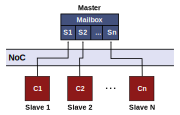
\includegraphics[width=\linewidth]{mailbox-concept.pdf}}%
				\hspace{1cm}%
				\subcaptionminipage[fig:mailbox-flow]%
					{.55\linewidth}%
					{Flow of execution: Slave sends a message, Master reads and notifies the sender.}%
					{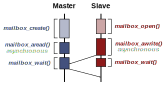
\includegraphics[width=\linewidth]{mailbox-flow.pdf}}%

				\fonte{Developed by the Author.}%
			\end{figure}

			% A Figura (fluxo) exemplifica o fluxo de comunicação entre um nó receptor e um emissor. A criação de uma Mailbox cria uma fila de mensagens vazia, onde os emissores são livres para enviar a primeira mensagem. Posteriormente, todos os envios necessitaram da permissão do receptor para que mensagens não sejam sobreescritas. Por este motivo, o receptor notificará o emissor ao consumir sua mensagem. A mensagem será copiada para um buffer do usuário e o espaço estará novamente disponível.

			% Teoricamente, a quantidade de mensagens permitidas por emissor pode ser de 1 à N. Entretanto, optou-se por permitir apenas 1 no Nanvix HAL devido as restrições de memória apresentada por manycores. E como o espaço é alocado estatícamente dentro do espaço de memória do kernel, permitir que o usuário escolhe-se o tamanho da fila de mensagem não reduziria o espaço prévio necessário. Todavia, o uso de uma mensagem é suficiente para programas servidores tratarem requisitações no nível do Multikernel. Por exemplo, a mensagem pode ser usada para codificar pequenas operações e sinais de controle do sistema.

			\autoref{fig:mailbox-flow} exemplifies the communication flow between a
			receiver and a sender node. The receiver creates an empty message queue
			where senders are free to send the first message. Subsequently, in order
			not to overwrite old messages, all transmissions require the permission
			of the receiver. For this reason,  when the receiver consumes a message,
			it copies the message to the user buffer, releases the queue space, and
			notifies the sender.
			
			Theoretically, the number of messages allowed per sender can be from
			$1$ to $N$. However, \nanvix \hal statically allocates sufficient
			memory for the message queue inside the kernel. Therefore, we chose
			to allow only one message due to memory constraints presented by
			lightweight manycores. Furthermore, using one message is sufficient	for
			servers to handle requests at the \multikernel level. For instance, the
			message can be used to encode small operations and system control signals.
			
			\subsubsection{Receiver Side Implementation}

% % Interface e seus parâmetros
% 				O código 3 apresenta a interface da Mailbox para um nó receptor. A criação de uma Mailbox requer que a aplicação informe o ID Lógico no nó local. Esta identificação é necessária por causa do múltiplos nós existentes nos Cluster I/O. As demais operações utilizam o identicador retornado na criação da mailbox. Para a leitura de uma mensagem, o usuário é obrigado a passar o local onde a mensagem será copiada e o tamanho a ser copiado. O tamanho é sempre constante mas é utilizado como verificação da integridade da operação. A cópia bem sucedida de uma mensagem liberará o escravo que executar a função de espera. Neste processo de liberação, o core mestre executa o flush da mensagem para a SRAM para que o escravo, ao invalidar a sua cache, possa ler a mensagem.

% % Recursos de hardware
% 				A Mailbox é mais complexa do que o Sync porque utiliza recursos DNoC e CNoC. Especificamente, o receptor necessita de 1 slot de recebimento da DNoC e 1 canal de transmissão da CNoC. A necessidade de 1 canal de transmissão durante toda a vida da Mailbox do receptor limita a criação de apenas 1 mailbox por nó NoC. O slot rx é configurado utilizando dois tamanhos. Um para o tamanho de uma mensagem, o qual gerará interrupções, e outro para o tamanho total buffer alocado para proteção. O buffer é alocado dentro da memória do kernel com espaço suficiente para receber 24 mensagens. A mensagem, propriamente dita, é composta por um cabeçalho identificando o emissor, um corpo contendo a mensagem útil e um rodapé com o mesmo identificador. O canal de transmissão, por sua vez, é utilizado após a cópia da mensagem útil para o buffer do usuário, notificando o ID do cabeçalho.

% % Desafios da implementação
% 				O paralelismo no recebimento das mensagens introduziu alguns desafios na leitura assíncrona do Mailbox como (i) cada mensagem gera uma interrupção, (ii) interrupções preemptadas por outras não encontraram os recursos da DNoC que emitiram a interrupção e (iii) não é possível verificar a quantidade de interrupções geradas por um recurso. Para burlar estas barreiras, foi implementado um comportamento similar ao envio preguiçoso. Primeiro, um contador global contendo a quantidade total de mensagens recebidas permite que o receptor copie mensagens recebidas antes de uma leitura. Segundo, caso não haja mensagens disponíveis, a cópia será realizada pelo próximo disparo do manipulador. Terceiro, para resolver o problema das interrupções preemptadas, sempre que um manipulador é disparado ele percorrerá a fila de mensagens conferindo os cabeçalhos e rodapés. Ao identificar uma mensagem válida, o manipulador incrementa o contador e altera o rodapé para um código especifico. Desta forma, não perdemos nenhuma mensagem por não tratar uma interrupção.

					\autoref{code:hal-mailbox-receiver} presents the Mailbox interface for
					Receiver Nodes. The multiples nodes in \ioclusters forces the application
					to inform the local node ID on the creation of the \mailbox. The other
					operations use the file descriptor returned by creation function.
					Consumption of a message requires the application to enter a buffer and
					message size. Although the size is constant, it is used to verify the
					integrity of the operation. Successful copying of a message will release
					the slave that performs the wait function. In the release protocol, the
					master core flushes the message to the SRAM so that the slave, when
					invalidating its cache, can read the message.
					
					\mailbox is more complicated than Sync in terms of hardware resources.
					Specifically, the receiver requires one \dnoc receiving slot and one \cnoc
					transfer channel. The need for one transfer channel for the lifetime
					of the receiver limits the creation of only one mailbox per \noc node.
					The receiving slot is configured using two sizes. One for the size of
					a message, which will generate interrupts, and one for the total buffer
					size allocated for protection. The buffer is allocated within kernel
					memory with sufficient space to receive 24 messages. The message
					itself is composed of a header identifying the sender, a body containing
					the useful message, and a footer for handler control. The transfer channel,
					in turn, is used after copying the useful message to the user buffer,
					notifying the header ID.
					
					Parallelism in receiving messages introduced some challenges in the
					asynchronous reading of Mailbox. Where (i) each message generates an
					interrupt, (ii) interrupts preempted by others did not find the \dnoc
					resources that issued the interrupt, and (iii) cannot verify the
					number of interrupts generated by a resource. A behavior similar to
					lazy transfer has been implemented to circumvent these difficulties.
					First, a global counter containing the total amount of messages
					received allows the receiver to copy received messages on the
					asynchronous read call. Second, if no messages are available, copying
					will be performed by the next triggered handler. Third, to solve the
					problem of preemptive interrupts, whenever a handler is triggered,
					it will traverse the message queue checking headers and footers.
					When identifying a valid message, the handler increments the counter
					and changes the footer to a specific code. This way, no message is
					lost because a single handler identifies messages not yet counted.

\begin{listing}[!tb]
\caption{Nanvix HAL: Mailbox Interface for Receiver Node.}
\label{code:hal-mailbox-receiver}
\begin{minted}{c}
/* @brief Creates a mailbox. */
int mailbox_create(int nodenum);

/* @brief Destroys a mailbox. */
int mailbox_unlink(int mbxid);

/* @brief Reads data asynchronously from a mailbox. */
ssize_t mailbox_aread(int mbxid, void * buffer, size_t size);

/* @brief Waits for an asynchronous operation to complete. */
int mailbox_wait(int mbxid);
\end{minted}
\fonte{Developed by the Author.}
\end{listing}

			\subsubsection{Sender Side Implementation}

% Interface e seus parâmetros
				% O código 3 apresenta a interface da mailbox para o nó emissor. A abertura de uma mailbox requer que a aplicação informe o ID lógico do nó que irá receber a mensagem. O identificador da mailbox retornado pela função de abertura é utilizada para configurar e controlar as demais funções. A função de envio, em especial, implementa o conceito de envio preguiçoso. Ou seja, o core mestre nunca ficará bloqueado caso a mailbox não tenha permissão para enviar a mensagem. Ele realiza o agendamento do envio setando valores nas estruturas internas do kernel e copiando a mensagem útil para um buffer local, no qual consta o identificador do emissor. A função de espera é a mesma função utilizada pelo nó receptor onde o núcleo escravo aguardaram bloqueado em um spinlock até receber a permissão de envio.

				\autoref{code:hal-mailbox-sender} displays the Mailbox Interface for
				Sender Nodes. Opening a mailbox requires the application to inform
				the receiver ID to allocate related resources. The send function,
				in particular, implements the concept of lazy transfer. So, the master
				core never blocks if the mailbox is not allowed to transfer the message.
				The wait function is the same function used by the receiver node where
				the slave core waits blocked until receiving the transfer permission.

				% If the sender attempts to send a message before the receiver has consumed
				% the previous message, the sender will be blocked waiting for the sender's notification.
				% In this way, flow control is guaranteed, and the sender will not overwrite
				% messages unread by the receiver.

\begin{listing}[!tb]
\caption{Nanvix HAL: Mailbox Interface for Sender Node.}
\label{code:hal-mailbox-sender}
\begin{minted}{c}
/* @brief Opens a mailbox. */
int mailbox_open(int nodenum);

/* @brief Closes a mailbox. */
int mailbox_close(int mbxid);

/* @brief Writes data asynchronously to a mailbox. */
ssize_t mailbox_awrite(int mbxid, const void * buffer, size_t size);

/* @brief Waits for an asynchronous operation to complete. */
int mailbox_wait(int mbxid);
\end{minted}
\fonte{Developed by the Author.}
\end{listing}

% Recursos de hardware
				% O lado emissor também exige a alocação de recursos das duas NoCs. Porém, os recursos são opostos ao do receptor, no qual serão alocados 1 slot rx da CNoC e 1 canal de transmissão da DNoC. O slot rx CNOC alocado é relativo ao ID do receptor para evitar que aberturas para receptores distintos conflitassem ao tentar alocar o mesmo slot. O canal de transmissão é alocado dinamicamente dentre os 4 disponíveis. Deste modo, a quantidade máximo de mailboxes abertas por nó é limitado pelo número de canais de transmissão.

				The sender implementation also requires the allocation of resources
				from both \nocs. However, the resources are opposite to the receiver,
				where it allocates one \cnoc receiving slot and one \dnoc transfer channel.
				The allocated \cnoc receiving slot is relative to the receiver ID to
				prevent conflicts among openings for distinct receivers. The transfer
				channel is dynamically allocated. Because it has fewer transfer channels
				than receiving slots, transfer channels limit mailbox openings to 4 per node.

		\subsection{Portal Abstraction}
		\label{sec.portal-abs}

			% \begin{figure}[!tb]
			% 	\centering%
			% 	\caption{Portal Abstraction Concept: Node 1 create a portal and notify Node 2 to transfer the data.}%
			% 	\label{fig:portal}%
			% 	\includegraphics[width=.65\textwidth]{.pdf}%
			% 	\fonte{Developed by the Author.}%
			% \end{figure}

% Apresentação do portal e o conceito.
			% Por fim, a abstração Portal permite que dois nós troquem quantidades arbitrárias de dados. A Figura (conceito) apresenta a ideia conceitual do portal, onde se assemelha a do POSIX Pipes com controle de fluxo. A cardinalidade das operações é sempre 1:1, onde um par de nós abre um canal unidirecional para transferência de dados. Porém, ao contrário do POSIX Pipes que define que o pipe existe apenas entre dois processos, o portal permite que o receptor se comunique com outros nós através de um mesmo canal. O emissor, por sua vez, poderá apenas se comunicar com um nó.

% Fluxo da operação
			% A Figura (fluxo) exemplifica o controle de fluxo proposto para o portal. Ao tentar transmitir dados ao receptor, o emissor blorqueará até que o receptor esteja apto à receber. O receptor, ao habilitar uma troca de dados de cada vez, configura a leitura e notifica o emissor. Deste modo, o controle de fluxo garante que o receptor não será sobrecarregado, não receberá dados sem que a DMA esteja devidamente configurada, e não sobrescreverá dados prévios. O ato de habilitar uma comunicação permite que o receptor escolha com qual nó deseja se comunicar.

			Finally, \textit{Portal Abstraction} allows two nodes to exchange arbitrary
			amounts of data. \autoref{fig:portal-concept} presents the conceptual idea
			of the \portal, which resembles that of \posix Pipes with flow control.
			The cardinality of operations is always $1:1$, where a pair of nodes opens
			a one-way channel for data transfer. However, unlike \posix Pipes, which
			defines that the pipe exists only between two processes, the \portal allows
			the receiver to communicate with other nodes through the same channel.
			The sender, in turn, can only communicate with one node.

			\autoref{fig:portal-flow} exemplifies the flow control of the \portal.
			When attempting to transmit data to the receiver, the sender will block
			until the receiver can accept it. By enabling one data exchange at a time,
			the receiver sets the readout and notifies the sender. In this way,
			the flow control ensures that the receiver will not be overloaded, will
			not receive data without properly configured \dma, and will not overwrite
			previous data. Allowing communication empowers the receiver to choose which
			communications to prioritize.

			\begin{figure}[!tb]
				\centering%
				\caption{Portal Abstraction Concept.}%
				\label{fig:portal}%

				\subcaptionminipage[fig:portal-concept]%
					{.32\linewidth}%
					{Conceptual Overview.}%
					{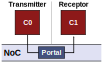
\includegraphics[width=\linewidth]{portal-concept.pdf}}%
				\hspace{1cm}%
				\subcaptionminipage[fig:portal-flow]%
					{.55\linewidth}%
					{Node 1 create a portal and notify Node 2 to transfer the data.}%
					{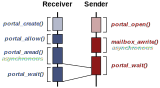
\includegraphics[width=\linewidth]{portal-flow.pdf}}%

				\fonte{Developed by the Author.}%
			\end{figure}

			\subsubsection{Receiver Side Implementation}

% Interface e seus parâmetros
				% O Código 5 apresenta a interface portal para nós receptores. Assim como a mailbox, a aplicação deve identificar o nó local para criar um portal. As demais funções utilizam o identificador do portal retornado pela função de criação. Para criar um canal de comunicação, o receptor sempre deverá executar 3 operações, allow, aread, wait. A função allow aloca um slot rx relativo ao nó remoto informado, limitando um canal por par de nós. Entretanto, a notificação apenas será enviada, relativo ao nó remote, após a configuração da DMA pela função aread. Por fim, o nó bloqueará na função wait até a comunicação ser completada.

% Recursos de hardware
				% Um portal receptor aloca um slot rx da DNoC e um canal tx da CNoC. Diferente da mailbox, o portal tem disponível 2 canais tx o que permite a criação de dois portais simultâneos. Tais portais não podem se comunicar com o mesmo nó ao mesmo tempo por causa da escolha do slot físico da DMA comentado no parágrafo anterior. A leitura configura o slot rx com o buffer e tamanho informado pela aplicação. Isto elimina as cópias intermediárias como da mailbox, onde a DMA escreve os dados direto no buffer da aplicação. As estruturas de controle também são simplificadas por causa disso contendo apenas flags e um spinlock liberado pelo manipulador do portal.

				\autoref{code:hal-portal-receiver} presents the Portal Interface for
				Receiver Nodes. Like the \mailbox, the application must identify the
				local node to create a \portal. The receiver must always perform
				three operations to perform communication, i.e., \textit{allow},
				\textit{read}, and \textit{wait}. The allow function allocates one
				receiving slot relative to the given remote node, limiting one
				channel per pair of nodes. However, the permission will only be
				sent after \dma configuration by the read function. Finally, the
				node will block in the wait function until receiving the informed
				data size.

				A Receiver allocates one \dnoc receiving slot and one \cnoc transfer
				channel. Unlike \mailbox, the \portal has two transfer channels
				available, which allows the creation of two simultaneous portals.
				Such portals cannot communicate with the same node at the same time
				because of the choice of the same physical slot. Read sets the
				receiving slot to the buffer and size informed by the application.
				The \dma eliminates intermediate copies like Mailbox because it
				writes data directly to the application buffer. Consequently,
				control structures have also been simplified, containing only
				control flags and the spinlock for asynchronous operations.

\begin{listing}[!tb]
\caption{Nanvix HAL: Portal Interface for Receiver Node.}
\label{code:hal-portal-receiver}
\begin{minted}{c}
/* @brief Creates a portal. */
int portal_create(int local);

/* @brief Destroys a portal. */
int portal_unlink(int portalid);

/* @brief Allow sender to transfer data. */
int portal_allow(int portalid, int remote);

/* @brief Reads data asynchronously from a portal. */
ssize_t portal_aread(int portalid, void * buffer, size_t size);

/* @brief Waits for an asynchronous operation to complete. */
int portal_wait(int portalid);
\end{minted}
\fonte{Developed by the Author.}
\end{listing}

			\subsubsection{Sender Side Implementation}

% Interface e seus parâmetros
				% O código 6 apresenta a interface portal para nós emissores. Na abertura de um portal, a aplicação é obrigada a informar o nó local e o nó remote que receberá os dados. O id local serve para distinguir a interface NoC casa haja multiplos nó em um cluster e o id do nó remote será utilizado para alocar e configurar o slot rx da CNoC que receberá a permissão de transferência. Isto garante que a permissão não será perdida, mesmo se a permissão chegar antes do emissor configurar a escrita. Os dados são transferidos seguindo o algoritmo de envio preguiçoso.

% Recursos de hardware
				% Os recursos de hardware necessários para abrir um portal são opostos ao recursos de criação. Especificamente, são necessários 1 slot rx da CNoC e 1 canal tx da DNoC. O slot rx está apto a receber a permissão desde a abertura do portal. O canal de transmissão é reservado mas só é utilizado quando for permitido o envio. Devido a limitação de 4 canais tx para o portal, apenas 4 portais emissores podem ser abertos ao mesmo tempo. A estruturas de controle para os portais emissores contém os parâmetros necessário para realizar o envio preguiçoso e um spinlock para controlar o término da operação de transferência.

				\autoref{code:hal-portal-sender} presents the Portal Interface for
				Sender Nodes. When opening a \portal, the application is required to
				inform the local node ID and the receiver node ID. The local ID serves
				to distinguish the NoC interface on \ioclusters. The receiver node ID
				identifies the \cnoc receiving slot that will catch the transfer
				permission. The early allocation ensures that the permission will not
				be lost even if the permission arrives before the sender sets up the
				transfer. The transfer configuration follows the lazy transfer algorithm.

				The hardware resources required to open a portal are the opposite of
				resources to create. Specifically, one \cnoc receiving slot and one
				\dnoc transfer channel are required. The transfer channel is reserved
				but only used when the transfer is allowed. Due to the limitation of
				four transfer channels to the portal, a node can open only four portals
				at a time. The control structures for the sender portals contain the
				parameters needed to perform the lazy transfer and a spinlock to
				asynchronous operations.

\begin{listing}[!tb]
\caption{Nanvix HAL: Portal Interface for Sender Node.}
\label{code:hal-portal-sender}
\begin{minted}{c}
/* @brief Opens a portal. */
int portal_open(int local, int remote);

/* @brief Closes a portal. */
int portal_close(int portalid);

/* @brief Writes data asynchronously to a portal. */
int portal_awrite(int portalid, const void * buffer, size_t size);

/* @brief Waits for an asynchronous operation to complete. */
int portal_wait(int portalid);
\end{minted}
\fonte{Developed by the Author.}
\end{listing}

				\todo[inline]{Trabalhos futuros: Eliminar a necessidade de informar o remote na abertura criando um função allow igual o reciever.}

	\section{User-Level Communication}
	\label{sec.comm-services}
	\todo{Or: Nanvix Microkernel Level}

		The inter-cluster communication module, described in \autoref{sec.low-level-comm},
		is designed to export a standard and straightforward communication
		primitives to different lightweight manycores.
		These primitives can be used by various types of \oss and applications.
		Thus, the module is flexible enough not to impact the performance
		of the upper layers negatively.
		For this, it does not provide rich management of the exposed abstractions.

		In this scenario, the communication services of \nanvix \microkernel seek
		to provide \ipc between distinct clusters.
		Specifically, these services perform the multiplexing of the hardware
		resources and the verification of the parameters that will be passed
		on the communication primitives.
		Due to the Master-Slave model, the responsibility of protecting,
		manipulating, and configuring \hal resources is of the master core.
		The slave core will request operations through the system call interface,
		passing the necessary information to the master.

		Considering that the abstractions make up the fundamental elements of
		the construction of more complex services, the \microkernel services
		were responsible for the management and multiplexing of the finite
		resources for the many cores of a cluster.
		In total, there are three communication services in the \nanvix \microkernel,
		each associated with an abstraction of the communication module,
		analogously named \sync, \mailbox, and \portal services.
		These services must take into account the memory constraints and the
		Master-Slave model chosen for the \microkernel.

		The impacts of the Master-Slave model, protection, management and manipulation 
		operations are similar to all services.
		Thereat, the following sections provide an overview of these topics punctuating 
		the differences of each service.

		They will be provided through interfaces that function as wrappers
		for the \hal abstraction functions.
		In the implementation of these interfaces, there will be a mapping
		between low-level identifiers, associated with \hal resources,
		and high-level identifiers, associated with resource protection structures.

			% The protection operations are mostly similar.
			% For instance, the use of unallocated resources, sanitizing entries,
			% checking valid identifiers, non-null pointers, and checking
			% for conflicting operations (reading in write-only resources).
			% In the meantime, there are exceptional cases in some services
			% that must be taken.
			% For instance, in the \sync service, a cluster cannot synchronize
			% with itself, or there is a repetition of identifiers in the
			% stipulated set of clusters.

			% Finally, some aspects of services and implementation still need
			% to be analyzed and will be better detailed in another version
			% of the dissertation.
			% For example, what resource multiplexing methods will be used
			% and their impacts on the Nanvix Microkernel services.

		\subsection{Impacts of the Master-Slave Model}

			O modelo mestre-escravo define que as estruturas internas do SO devem ser exclusivamente manipuladas pelo núcleo mestre.
			Para isso, cada serviço possui estruturas genéricas e simples que guardam flags de controle, parâmetros para identificação da recurso e armazenamento dos descritores físicos retornados pela HAL.
			Desta forma, existem dois conjuntos de funções que separa a responsabilidade dos escravos das responsabilidades do mestre.
			A única excessão é a chamada da função de esperar onde ela é inteiramente realizadas pelo núcleo escravo.
			Inclusive, foi possível exportar funções síncronas do lado do escravo ao forçar a espera da conclusão de operações assíncronas em uma chamada de sistema.

			O conjunto de funções do mestre segue a notação \texttt{kernel\_\textbf{abstraction}\_\textit{operation}} e é utilizada pelo mecanismo de chamadas de sistemas para realizar a proteção, manuseio e multiplexação dos serviços.
			O conjunto de funções destinada aos escravos é a interface exportada pelas chamadas de sistemas, definidas como \texttt{k\textbf{abstraction}\_\textit{operation}}.
			Suas responsabilidades é pesquisar qual identificado anexo ao nó local, caso exista mais de um, e realizar os testes de sanidade possíveis do lado do escravo.

			O fato de que o mestre não pode bloquear a espera de uma única operação forçou que a operação da chamada de espera seja realizada pelo escravo.
			Neste ponto, o escravo precisa acessar a estrutura interna do SO para consultar o descritor de baixo nível da abstração para que tenha acesso ao spinlock da HAL.
			Para garantir a coerência da estrutura, o mestre atualiza a memória local sempre que uma modificação é realizada e o escravo invalida sua cache.

		\subsection{Protection and Management}

			As operações de proteção e gerência envolvem duas fases, a fase do escravo e a fase do mestre.
			Na fase do escravo é verificado todos os problemas que poderiam ser detectados antes de requisitar a operação ao mestre.
			Por exemplo,
			(i) descritores de arquivos válidos,
			(ii) ponteiros de buffer não nulos,
			(iii) tamanhos de buffers dentro do limite estipulado, e
			(iv) a semântica dos serviços como sincronização consigo mesmo.
			
			O mestre, além de realizar as mesmas verificações do escravo, tem a responsabilidade de conferir a semântica das operações sobre um determinado recurso.
			Especificamente, o mestre
			(i) identifica multiplas criações/aberturas
			(ii) verifica operações conflitantes, como escritas em recursos configurados apenas para leitura,
			(iii) mensura tempo de comunicação e quantidade total de bytes transmitidos/recebidos, e
			(iv) chama as abstrações da HAL identificando erros retornados.

		\subsection{Multiplexing}

			A identificação de recursos criados/abertos com os mesmo argumentos permite que multiplos escravos utilizem um mesmo recurso em momentos distintos.
			Para isso, as estruturas internas do SO guardam, da forma mais simplificada possível, os argumentos utilizados na criação/abertura de um serviço.
			Quando identificado os mesmos argumentos, um contador de referências é incrementado.
			O mestre configura o recurso como ocupado quando solicitado uma leitura/escrita.
			Um segundo escravo que deseja ler/escrever será impedido até que a operação anterior seja concluida.
			A liberação dos recursos da HAL só seram liberados quando todas as referências forem removidas.

		\subsection{Input/Output Control}

			Os serviços de mailbox e portal contam com uma chamada de sistema especial, chamada de \ioctl.
			Essas chamada concede a implementação de operações que não podem ser expressadas por chamadas de sistemas regulares.
			No caso dos serviços de comunicação, 2 tipos de operações foram implementadas.
			A primeira operação, denominada \texttt{IOCTL\_GET\_VOLUME} consulta a quantidade atual de bytes transmitidos/recebidos de um serviço.
			A segunda operação, denominada \texttt{IOCTL\_GET\_LATENCY}, consulta a soma das latências das comunicações mensuradas através da diferença de duas leituras de clock.
			Essa chamada de sistema pode ser extendida futuramente para introduzir novas funcionalidades e operações sem causar mudanças nas interfaces atuais.

		\subsection{Validation and Correctness Tests}

			A validação e teste de corretude da implementação dos serviços foi realizada através de 2 conjunto de testes unitários, testes de API e testes de FALHA, respectivamente.
			Por um lado, os testes de API criam, abrem e estimulam os serviços com argumentos dentro dos intervalos de valores válidos.
			Por outro lado, os testes de FALHA utilizam argumentos fora do intervalo de domínio das operações.
			A falha deve gerar um valor de erro previamente conhecido.
			Os testes validam qualquer mudança feita verificando todos os comportamentos esperados pelos serviços.

\chapter{Experiments}
\label{ch.experiments}

    In this Chapter, ...

    \section{Micro-benchmarks}

        \subsection*{Ping-Pong}

            In this benchmark, I will write about ...

        \subsection*{Broadcast}

            In this benchmark, I will write about ...

        \subsection*{Scather}

            In this benchmark, I will write about ...

        \subsection*{Gather}

            In this benchmark, I will write about ...

        \subsection*{All-Gather}

            In this benchmark, I will write about ...

    \section{Results}

        In this section, I will write about ...
\chapter{Schedule}
\label{ch.schedule}

This chapter presents the schedule for the next activities
planned for the development of the undergraduate dissertation.

\section{Activities}
\label{sec:gantt}

\begin{figure}[!h]
	\caption{Chart Gantt of the Schedule.}

	\begin{center}
		\begin{ganttchart}[
			x unit=0.6cm,
			y unit title=0.6cm,
			y unit chart=0.6cm,
			hgrid,
			vgrid={{dotted, dotted, dotted, dotted, dotted, dotted}},
			% title label font=\3scriptsize,
			title/.append style={fill=gray!30},
			title height=1,
			bar/.append style={fill=gray!30,rounded corners=2pt},
			bar label font=\scriptsize,
			group label font=\scriptsize,
		]{7}{12}

		\gantttitle{\textbf{Meses}}{6} \\
		\gantttitle{\textbf{2019}}{6} \\
		\gantttitlelist{7,8,9,10,11,12}{1} \\
		\ganttbar{1. Writing the Implementation and Experiments.}{7}{9} \\
		\ganttbar{2. In-depth Writing of the Proposal.}{9}{10} \\
		\ganttbar{3. Presentation of the Undergraduate Dissertation.}{11}{11} \\
		\ganttbar{4. Review and Final Submission of the Undergraduate Dissertation.}{12}{12} \\

		\end{ganttchart}
	\end{center}

	\label{chart.gantt}
\end{figure}

	Figure \ref{chart.gantt} shows the planned activities and their durations visually.
	Beginning in July 2019, the final submission is planned for December 2019.
	In detail, the activities are described below:

	\begin{itemize}
		\item \textit{Writing the Implementation and Experiments:}
			Currently, the inter-cluster communication module has the \sync abstraction
			completed and part of the \mailbox abstraction.
			Since the \portal abstraction uses the same low-level mechanisms of the others
			abstractions, its implementation will be facilitated.
			The communication services already have prototypes developed by the author
			for a symmetric \os.
			In this way, the prototypes will need to be modified to use the \hal and
			modified for a master-slave model.
			Finally, micro-benchmarks will be developed to perform an analysis of the
			performance of the implemented services.
		\item \textit{In-depth Writing of the Proposal:}
			During September and October, this activity will be committed to improving
			this draft and detailing the project decisions chose and implementations produced.
			We will also describe the experiments performed and discuss the results obtained.
		\item \textit{Presentation of the Undergraduate Dissertation:}
			November will be dedicated to the development and preparation of the presentation
			of the work and the results achieved.
			So finally, to present the dissertation to the evaluators.
		\item \textit{Review and Final Submission of the Undergraduate Dissertation:}
			Finally, December will be dedicated to the correction of the issues indicated
			by the evaluators and finalized with the final submission of the dissertation.
	\end{itemize}

 \chapter{Conclusions}
\label{ch.conclusions}

Iniciamente, este trabalho apresentou um contexto histórico
dos processadores multicores até os tempos atuais.
Ao demonstrar a relação entre o aumento de núcleos e o consumo
de energia, foi discutido como a academia e a industria
começaram a desenvolver alternativas para amenizar as
barreiras tecnológicas que surgiram.
Contudo, mesmo os novos processadores que surgiram
se destacarem por causa do seu desempenho e consumo energético,
eles pecam em programabilidade e portabilidade proveniente
das suas características arquiteturais, tais como, modelo de
programação híbrido, subsistemas de memória restritivos,
falta de coerência de cache e configurações heterogênicas.
Parte das dificuldades deriva da incompletudo dos sistemas operacionais
e runtimes existentes em lidar com as severas restrições arquitetônicas.

Neste trabalho será desenvolvido um módulo de comunicação entre cluster
projetado em torno dos principais pontos no desenvolvimento de um
sistema operacional.
Como base, foi discutido aspectos de hardware e softwares
de arquiteturas paralelas e distribuidas.
Foram apresentadas modelos distintos de abordagens de sistemas operacionais
que podem a vir utilizar o módulo de comunicação.
Deste modo, para fornecer o esqueleto básico para tais sistemas operacionais,
três abstrações de comunicação foram propostas para a HAL com a preocupação
de prover qualidade de serviço.
Entre elas estão a abstração sync para criar barreiras distibuidas.
A abstração mailbox fornece a troca de mensagens pequenas com controle 
de fluxo.
E por fim, a abstração portal possibilita a troca de quantidade arbitrárias
de dados entre dois clusters.

Outra contribuição deste trabalho apresentada foram os 
serviços de comunicação para um sistema operacional baseado na abordagem microkernel.
Esses serviços providenciam a multiplexação dos recursos expostos pela HAL
e a verificação dos parâmetros necessários para cada abstração.
De forma geral, esses serviços exportam uma forma segura ao usuário
se beneficiando da não concorrência das estruturas internas do SO 
por causa da separação de responsabilidades de mestre e escravo.
Por fim, a proposta detalhou, de forma geral, vários aspectos
das implementações.
Devido ao fato dos serviços dependerem do módulo de comunicação da HAL
para serem desenvolvido, os tópicos associados ao módulo acabaram sendo
mais detalhados e melhor explorados.
Entretanto, a próxima versão da dissertação especificará com maior clareza
e objetividade ambas as contribuições deste trabalho.


\postextual%
% Assume-se que \postextual já foi feito

\apendices

\chapter{Scientific article}
\label{ch:article}

\includepdf[scale=1,pages=-,pagecommand={}]{pos-textual/erad20.pdf}
\chapter{Source Code}
\label{ch:source-code}

% \let\svaddcontentsline\addcontentsline
% \renewcommand\addcontentsline[3]{%
%   \ifthenelse{\equal{#1}{lof}}{}%
%   {\ifthenelse{\equal{#1}{lot}}{}{\svaddcontentsline{#1}{#2}{#3}}}}

% \renewcommand\thefigure{\thesection.\arabic{figure}}

% \counterwithin{figure}{section}

\renewcommand{\thefigure}{B-\arabic{figure}}
\setcounter{figure}{0}

\section{Nanvix Project Structure}

    The development of a general-purpose distributed operating system for
    lightweight manycores processors, called \nanvixos, includes the source
    code for this undergraduate dissertation. \nanvixos is the result of an
    open-source, collaborative project made available on the Github platform.
    Since it is not semantically interesting to have only part of the source
    code and it is impossible to insert all OS code into this document, this
    appendix details where find and test the developed code. The Nanvix
    Project is detailed in \autoref{sec.nanvix}.

    Specifically, there is a separate Github repository for each abstraction
    layer that is maintained and updated by Nanvix contributors. Submodules,
    supported by the git tool, create an implicit dependency hierarchy
    between the Nanvix repositories. Thus, each layer that depends on another
    has guarantees of its operation and is exempt from its implementation.
    Theses guarantees make the codes better manageable, modular, and better
    portable. All repositories contain test sets (Validation and Fault tests)
    to ensure the correct implementation of exported interfaces on the several
    supported architectures.

    All repositories follow a branch naming convention, where only two
    branches are, in fact, essential. First, the master branch contains
    the most stable version of the system and marks the significant
    releases of Nanvix versions. Second, the unstable branch contains
    the most current version, but there may still exist bugs or required
    parts missing. The other branches are intended to implement new features,
    improve existing ones, or fix bugs. These other branches are merged
    into the unstable branch when passing all regression tests.

    The following subsections, ordered by dependency, detail the four
    repositories that contain the source code of this undergraduate dissertation.

    \subsection{Microkernel-Benchmarks}
    
        The \textit{Microkernel-Benchmarks} implements the micro-benchmarks
        that stimulate communication services. Specifically, there are four
        micro-benchmarks for each data transfer service, detailed in
        \autoref{sec.evaluation-methodology}. In this repository, there
        are also scripts for compiling and running experiments on the
        \mppa platform.

        The developed code version are available at
        \url{https://github.com/joaovicentesouto/microkernel-benchmarks},
        in the \textit{collective-comm-routines branch} or, especificaty,
        in the \textit{commit aafd9a70f8188105efabd651050bc7cafc39d343}.
        \autoref{fig:tree.benchs} presents, in the form of a file system
        tree, all files that are fully, or partially, developed. The
        \textit{include} folder contains only one file with static
        experiment settings. The \textit{src} folder is made up of
        auxiliary files and the micro-benchmarks themselves.

        \begin{figure}[!ht]
            \centering%
            \begin{forest}
            for tree={
                grow'=0,
                parent anchor=children,
                child anchor=parent,
                anchor=parent,
            },
            where level=0{
                draw
            }{
                if={(n()==1)&&(level()>1)}{
                calign with current edge
                }{},
                if n children=0{folder}{},
                edge path'={(!u.parent anchor) -- ++(5pt,0) |- (.child anchor)},
            }
            [microkernel-benchmarks
                [include
                    [kbench.h]
                ]
                [src
                    [utils
                        [args.c]
                        [barrier.c]
                        [crt0.c]
                        [node.c]
                        [results.c]
                        [string.c]
                        [times.c]
                    ]
                    [mailbox
                        [allgather/main.c]
                        [broadcast/main.c]
                        [gather/main.c]
                        [pingpong/main.c]
                    ]
                    [portal
                        [allgather/main.c]
                        [broadcast/main.c]
                        [gather/main.c]
                        [pingpong/main.c]
                    ]
                ]
            ]
            \end{forest}%
            \caption{Source tree.}%
            \label{fig:tree.benchs}%
        \end{figure}

    \subsection{LibNanvix}

        LibNanvix defines and exports user interfaces for Nanvix Microkernel
        services. Implementations, in turn, have the responsibility of making
        requests to the master core through the kernel call interface exported
        by the microkernel repository, detailed in \autoref{sec.microkernel}.
        Briefly, this repository is the complement of the Microkernel repository.

        \autoref{fig:tree.libnanvix} illustrates, as a file system tree,
        all files developed of the communication abstraction user
        interface. First, the files in the \textit{include} folder
        define the user interfaces. Second, files within the
        \textit{ikc} folder perform checks to identify potential
        problems. Finally, the test folder contains the validation
        and correctness tests of user abstractions. The code version
        is available in \textit{commit a9dcb35dd8727aefe41d316ac2609c88073e160e}
        at \url{https://github.com/nanvix/libnanvix}.

        \begin{figure}[!ht]
            \centering%
            \begin{forest}
            for tree={
                grow'=0,
                parent anchor=children,
                child anchor=parent,
                anchor=parent,
            },
            where level=0{
                draw
            }{
                if={(n()==1)&&(level()>1)}{
                calign with current edge
                }{},
                if n children=0{folder}{},
                edge path'={(!u.parent anchor) -- ++(5pt,0) |- (.child anchor)},
            }
            [libnanvix
                [include/nanvix
                    [mailbox.h]
                    [noc.h]
                    [portal.h]
                    [sync.h]
                ]
                [src
                    [libnanvix/ikc
                        [mailbox.c]
                        [noc.c]
                        [portal.c]
                        [sync.c]
                    ]
                    [test
                        [kmailbox.c]
                        [knoc.c]
                        [kportal.c]
                        [ksync.c]
                    ]
                ]
            ]
            \end{forest}%
            \caption{Source tree.}%
            \label{fig:tree.libnanvix}%
        \end{figure}

    \subsection{Microkernel}
    
        implements of part of the asynchronous microkernel
        detailed in \autoref{sec.microkernel}. This repository contains all
        internal \os structures and the implementation of master-side calls.
        Available at \url{https://github.com/nanvix/microkernel}.

        % \begin{itemize}
        %     \item Microkernel: a9826dec62baa3fe47ab3a77b15f3ccfdd84b79a
        %     \item microkernel/include/nanvix/mailbox.h
        %     \item microkernel/include/nanvix/noc.h
        %     \item microkernel/include/nanvix/portal.h
        %     \item microkernel/include/nanvix/syscall.h
        %     \item microkernel/src/kernel/noc/mailbox.c
        %     \item microkernel/src/kernel/noc/portal.c
        %     \item microkernel/src/kernel/noc/sync.c
        % \end{itemize}
        \begin{figure}[!ht]
            \centering%
            \begin{forest}
            for tree={
                grow'=0,
                parent anchor=children,
                child anchor=parent,
                anchor=parent,
            },
            where level=0{
                draw
            }{
                if={(n()==1)&&(level()>1)}{
                calign with current edge
                }{},
                if n children=0{folder}{},
                edge path'={(!u.parent anchor) -- ++(5pt,0) |- (.child anchor)},
            }
            [microkernel
                [include/nanvix
                    [mailbox.h]
                    [noc.h]
                    [portal.h]
                    [sync.h]
                ]
                [src/kernel/noc
                    [mailbox.c]
                    [portal.c]
                    [sync.c]
                ]
            ]
            \end{forest}
            \caption{Source tree.}
        \end{figure}

    \subsection{HAL}
    
        defines and implements the interfaces of the lowest level
        abstractions. This repository deals directly with the multiple
        supported architectures, including \mppa, \optimsoc, \hero, and a
        \unix implementation for testing. More details in \autoref{sec.hal}.
        Available at \url{https://github.com/nanvix/hal}.

        % \begin{itemize}
        %     \item HAL: 1e7d3bc64decff023ac91cdecc2e0ac6c53ac946
        %     \item hal/include/nanvix/hal/target/mailbox.h
        %     \item hal/include/nanvix/hal/target/portal.h
        %     \item hal/include/nanvix/hal/target/sync.h
        %     \item hal/include/nanvix/hal/processor/clusters.h
        %     \item hal/include/nanvix/hal/processor/noc.h
        %     \item hal/include/arch/target/kalray/mppa256/mailbox.h
        %     \item hal/include/arch/target/kalray/mppa256/portal.h
        %     \item hal/include/arch/target/kalray/mppa256/sync.h
        %     \item hal/include/arch/processor/bostan/clusters.h
        %     \item hal/include/arch/processor/bostan/noc.h
        %     \item hal/include/arch/processor/bostan/noc/tag.h
        %     \item hal/include/arch/processor/bostan/noc/ctag.h
        %     \item hal/include/arch/processor/bostan/noc/dtag.h
        %     \item hal/include/arch/processor/bostan/noc/dma.h
        %     \item hal/src/hal/arch/target/mppa256/mailbox.c
        %     \item hal/src/hal/arch/target/mppa256/portal.c
        %     \item hal/src/hal/arch/target/mppa256/sync.c
        %     \item hal/src/hal/arch/processor/bostan/clusters.c
        %     \item hal/src/hal/arch/processor/bostan/noc.c
        %     \item hal/src/hal/arch/processor/bostan/ctag.c
        %     \item hal/src/hal/arch/processor/bostan/dtag.c
        %     \item hal/src/hal/arch/processor/bostan/dma.c
        %     \item hal/src/test/target/mailbox.c
        %     \item hal/src/test/target/portal.c
        %     \item hal/src/test/target/sync.c
        %     \item hal/src/test/processor/clusters.c
        %     \item hal/src/test/processor/cnoc.c
        %     \item hal/src/test/processor/dnoc.c
        %     \item hal/src/test/processor/noc.c
        % \end{itemize}
        \begin{figure}[!ht]
            \centering%
            \begin{forest}
            for tree={
                grow'=0,
                parent anchor=children,
                child anchor=parent,
                anchor=parent,
            },
            where level=0{
                draw
            }{
                if={(n()==1)&&(level()>1)}{
                calign with current edge
                }{},
                if n children=0{folder}{},
                edge path'={(!u.parent anchor) -- ++(5pt,0) |- (.child anchor)},
            }
            [hal
                [include
                    [nanvix/hal
                            [processor
                                [noc.h]
                                [clusters.h]
                            ]
                            [target
                                [mailbox.h]
                                [portal.h]
                                [sync.h]
                            ]
                    ]
                    [hal/arch
                        [processor/bostan
                            [noc.h]
                            [clusters.h]
                            [noc
                                [tag.h]
                                [ctag.h]
                                [dtag.h]
                                [dma.h]
                            ]
                        ]
                        [target/kalray/mppa256
                            [mailbox.h]
                            [portal.h]
                            [sync.h]
                        ]
                    ]
                ]
                [src
                    [hal/arch
                            [processor/bostan
                                [dma.c]
                                [noc.c]
                                [ctag.c]
                                [dtag.c]
                                [clusters.c]
                            ]
                            [target/mppa256
                                [mailbox.c]
                                [portal.c]
                                [sync.c]
                            ]
                    ]
                    [test
                        [processor
                            [noc.c]
                            [cnoc.c]
                            [dnoc.c]
                            [clusters.c]
                        ]
                        [target
                            [mailbox.c]
                            [portal.c]
                            [sync.c]
                        ]
                    ]
                ]
            ]
            \end{forest}
            \caption{Source tree.}
        \end{figure}

    % The links to access each of the repositories are:

    % \begin{description}
    %     \item[Microkernel-Benchmarks] \url{https://github.com/joaovicentesouto/microkernel-benchmarks/tree/collective-comm-routines}
    %     \item[LibNanvix] \url{https://github.com/nanvix/libnanvix}
    %     \item[Microkernel] \url{https://github.com/nanvix/microkernel}
    %     \item[HAL] \url{https://github.com/nanvix/hal}
    % \end{description}

\section{Exemplo de executação dos testes de regressão}
\label{sec:code-example}

O Código X exemplifica o download do código fonte da LibNanvix, sua compilação para a plataforma MPPA, e a executação dos testes de regressão.

% \begin{description}
    
% \end{description}

% export TARGET=mppa256
% cd $HOME
% git clone --recursive https://github.com/nanvix/libnanvix.git $HOME/libnanvix
% cd libnanvix
% git submodule update --init --recursive
% make contrib
% make all
% make run-ccluster KERNEL=hello-world

\imprimirglossario

\imprimirindice


%%% Local Variables:
%%% mode: latex
%%% TeX-master: "main"
%%% End:


\bibliography{references}

\end{document}
